%\documentclass[11pt]{article}
\documentclass[conference]{IEEEtran}
\usepackage{tikz}

\usepackage[utf8]{inputenc}
\usepackage[noheadfoot, margin=1in ]{geometry}

\usepackage{amsmath} \usepackage{amsthm} \usepackage{amsfonts} \usepackage{amssymb} 

%\usepackage{mathtools}
\usepackage{graphicx}
\usepackage{relsize}
\usepackage{xy}
\input{xypic}
\usepackage{bbm}
\setlength{\footskip}{20pt}

\usepackage{enumerate}

\onecolumn

\theoremstyle{plain}
\newtheorem{thm}{Theorem}
\newtheorem{prop}{Proposition}
\newtheorem{lem}{Lemma}
\newtheorem{corollary}{Corollary}
\newtheorem{claim}{Claim}


\theoremstyle{definition}
\newtheorem{definition}{Definition}
\newtheorem{example}{Example}
\newtheorem{conjecture}{Conjecture}
\newtheorem{question}{Question}
\newtheorem{problem}{Problem} \newtheorem*{prob*}{Problem}

\theoremstyle{remark}
\newtheorem{rem}{Remark}
\newtheorem{rems}{Remarks}
\newtheorem{para}{}
\newtheorem{summary}{Summary}



\renewcommand{\Re}[1]{\ensuremath{\operatorname{Re}\left\{#1\right\}}}
\renewcommand{\Im}[1]{\ensuremath{\operatorname{Im}\left\{#1\right\}}}

\newcommand{\BigO}[1]{\ensuremath{\operatorname{O}\bigl(#1\bigr)}}

\global\long\def\Z{\mathrm{{\bf Z}}}
\global\long\def\N{\mathrm{{\bf N}}}
\global\long\def\Gal{\mathrm{Gal}}





\global\long\def\RR{\mathbb{R}}
\global\long\def\CC{\mathbb{C}}
\global\long\def\NN{\mathbb{N}}
\global\long\def\QQ{\mathbb{Q}}
\global\long\def\ZZ{\mathbb{Z}}
\global\long\def\EE{\mathbb{E}}
\global\long\def\PP{\mathbb{P}}
\global\long\def\FF{\mathbb{F}}

 \global\long\def\dd{\cdots}
\global\long\def\normal{\triangleleft}

\newcommand*{\Scale}[2][4]{\scalebox{#1}{\ensuremath{#2}}}%




\begin{document}

\title{Beyond Group Codes: Point-to-point and Multi-Terminal Settings}

\maketitle


\section{Introduction}





\section{Preliminaries}

\paragraph{ \textbf{Groups}} 
A group is a set $\bf H$ equipped with a binary operation $``+"$. We denote such group by $(\bf H,+)$. All groups considered in this paper are \textit{Abelian groups}, i.e., the group operation is commutative. A subset $\bf M$ of $\bf H$ is a \textit{subgroup} and it is denoted by $\bf M \leq H$, if it is closed under the group operation. For a subgroup $\bf M$ in $\bf H$, define a \textit{coset} to be a shift of $\bf M$ by an element $a\in \bf H$. Given a subgroup $\mathbf{M} \leq \mathbf{H}$ and for any $a \in \mathbf{H}$, define $[a]_{\mathbf{M}}:=g+\mathbf{M}$. Let $\mathbf{S} \subseteq \mathbf{H}$ be a subset; $\mathbf{S}$ is a \textit{left transversal} for $\mathbf{M}$ in $\mathbf{H}$ if and only if every coset of $\mathbf{M}$ contains exactly one element of $\mathbf{S}$. 


\paragraph{\textbf{Group Codes}}
Consider a group $\bf H$. A group code $\mathcal{C}$ with length $n$ is a subgroup of $\bf H^n$; where $\mathbf{H}^n$ is the group with $n$ times Cartesian product of $\mathbf{H}$ as a set and element-wise addition as a group operation. A shifted group code is a translation of $\mathcal{C}$ by an element $b^n\in \bf H^n$. The ensemble of group codes is the collection of all subgroups of $\mathbf{H}^n$. Aria \textit{et.al.} \cite{Aria-group} characterized such ensemble. 


\paragraph{\textbf{Discrete Memoryless Channel}}
 $(\mathcal{X},\mathcal{Y}, W_{Y|X})$ denotes a discrete memory-less channel with input alphabet $\mathcal{X}$, output alphabet $\mathcal{Y}$ and conditional probability distribution $W_{Y|X} \in \mathcal{P}(X|\mathcal{Y})$. The \textit{Symmetric Channel Capacity} for such channel is defined to be the mutual information $I(X;Y)$ when $X$ is a uniform random variable taking values from $\mathcal{X}$ and $Y$ is the out put of the channel.
 
\paragraph{\textbf{Discrete Memoryless Source}}
We consider only discrete-time memoryless sources, in this paper. The source is modeled by a random process $X$ taking values from a set $\mathcal{X}$ with probability distribution $P_X$. The reconstructed source is denoted by another random process $Z$ taking values from $\mathcal{Z}$. The reconstruction is measured by a distortion measure $d: \mathcal{X} \times \mathcal{Z} \rightarrow [0,\infty]$. Such source is denoted by $(\mathcal{X}, \mathcal{Z}, P_X,d)$. The \textit{Symmetric Rate-distortion Function} for such source is defined as 

\begin{equation*}
R(D)=\min_{P_{Z|X}: \EE\{d(X,Z)\}\leq D} I(X;Z)
\end{equation*}
where $Z$ needs to be uniform over $\mathcal{Z}$.



\section{Pseudo-Group Codes } \label{sec: pseudo+group}
In this section a new coding scheme called \textit{Pseudo-group code} is proposed. The coding scheme consists of multiple layers of codes. The first layer is a group code. The other layers are not group codes, but they retain some algebraic structures. Therefore, pseudo-group codes obtain looser algebraic structures than group codes; in particular, only a part of a pseudo-group code is a group code. 

Assume $r$ is a positive integer and $p$ is a prime number. In what follows, the construction of a pseudo-group code for the underlying group $\ZZ_{p^r}=\{0,1,\cdots, p^r-1\}$ with addition as the group operation is proposed.

Given a positive integer $n$, a pseudo-group code with length $n$ over the underlying group $\ZZ_{p^r}$ consists of $r$ layers of cods. For $i \in \{0,1,\cdots,r-1\}$, the $i^{th}$ layer has the generator matrix $\mathbf{G}_i$ of dimension $k_i\times n$ with elements belonging to $\ZZ_{p^r}$. Let $p^{r-i}\ZZ_{p^r}=\{0, p^{r-i}, 2\cdot p^{r-i}, \cdots, (p^{i}-1) \cdot p^{r-i}\}$ and $T_i=\{0,1,\cdots, p^{r-i}-1\}$. Therefore, $T_i$ is a transversal for the subgroup $p^{r-i}\ZZ_{p^r}$ in $\ZZ_{p^r}$. Define the code-book of the $i^{th}$ layer as: 

\begin{equation}\label{eq: pseudo group codes layer i}
\mathcal{C}_i=\{ u_i^{k_i}\mathbf{G}_i: u_i^{k_i}\in T_i^{k_i}\}
\end{equation}

Now the pseuso-group code is defined as:
\begin{equation}\label{eq: pseudo group codes}
\mathcal{C}=\sum_{i=0}^{r-1} \mathcal{C}_i+b^n
\end{equation}

Where the summation is element-wise and $b^n\in \ZZ_{p^r}^n$ is a dither vector. The rate of this code is  
\begin{equation}
R=\sum_{i=0}^{r-1} \frac{k_i}{n} \log_2 |T_i| = \sum_{i=0}^{r-1} \frac{k_i}{n} (r-i) \log_2 p
\end{equation}
There is an alternative representation for the above pseudo-group code. Let $\mathbf{J}=\prod_{i=0}^{r-1}T_i^{k_i}$ and define the map 
\begin{align}\label{eq: phi}
&\phi :\mathbf{J} \rightarrow \ZZ_{p^r}^n\\\nonumber
& \phi(\mathbf{a}):=\sum_{i=0}^{r-1} u_i^{k_i}\mathbf{G}_i 
\end{align}

where $\mathbf{a}=(u_0^{k_0},u_0^{k_1}, \cdots, u_{r-1}^{k_{r-1}})$ is an element of $\mathbf{J}$. Therefore, $\mathcal{C}$ is the image of $\phi$ that is translated by the vector $b^n$. In this paper,  we refer to code-words of $\mathcal{C}$ by $\phi(\mathbf{a})+b^n$ .

For fixed $n$ and $k_i$, the random ensemble of pseudo-group codes consists of all codes of the form $\mathcal{C}$ where elements of the generator matrices $\mathbf{G}_i$ and dither vector $b^n$ are chosen independently of each other and uniformly from the set $\ZZ_{p^r}$.


The above construction provides a coding strategy with multiple structured layers of codes. Such layered framework helps pseudo-group codes obtain more flexibility to match the structure of a channel or source as a channel coding or source coding, respectively. Such frameworks achieve the information theoretical limits in some point-to-point settings. It will be shown later in this paper, that pseudo-group codes outperform group codes. In fact, they achieve the symmetric channel capacity and symmetric rate-distortion function in certain point-to-point problems. The next section shows the achievable rate of pseudo-group codes for discrete memory-less channels.  





\section{Channel Coding}

Let $(\mathcal{X},\mathcal{Y}, W_{Y|X})$ denote a discrete memoryless channel with input alphabet $\mathcal{X}$, output alphabet $\mathcal{Y}$ and conditional probability distribution $W_{Y|X} \in \mathcal{P}(X|\mathcal{Y})$. In addition, suppose that $\mathcal{X}=\ZZ_{p^r}$ where $r$ is a positive integer and $p$ is a prime number. An achievable rate for the ensemble of the group codes over such channel is derived in \cite{Aria-group 2}.


\begin{thm}\label{thm: group codes channel}
 Suppose $X$ is a random variable with uniform distribution over $\ZZ_{p^r}$. For any integer $0\leq s \leq r-1$, let $[X]_{s}=X+M_s$; where $M_s = p^s\ZZ_{p^r}$ is a subgroup of $\ZZ_{p^r}$. The ensemble of the group codes achieves the following bound for the channel $(\mathcal{X}=\ZZ_{p^r},\mathcal{Y}, W_{Y|X})$:

\begin{equation*}
R_{g,c.c.}\leq \min_{s=0}^{r-1} \frac{r}{r-s} I(X;Y|[X]_{s})
\end{equation*}
\end{thm}


%%%%%%%define $\mathbf{s}=(1,2, \cdots, r)$. Also define the vectors $\mathbf{\beta, t} $ and $\mathbf{b}$ as the following:
%%%%%%%
%%%%%%%$\mathbf{\beta}=(\beta_i)_{i=1}^r$ such that $\sum_{i=1}^r \beta_i=1, \beta_i \geq 0$
%%%%%%%
%%%%%%%$\mathbf{t}=(t_i)_{i=1}^r$ such that $0 \leq t_i \leq i$
%%%%%%%
%%%%%%%$\mathbf{b}=(b_i)_{i=1}^r$ with $b_i \in \ZZ_{p^r}$
%%%%%%%
%%%%%%%Define $\mathbf{\eta}=(\eta_{i,j})_{i,j =1}^r$ with $\eta_{i,j}$ as integers that satisfy $0\leq \eta_{i,j}\leq min(i,j)$. 
%%%%%%%
%%%%%%%$\omega_{t}=\frac{\sum_{i=1}^r t_i \beta_i \log_2 p}{\sum_{i=1}^r i \beta_i \log_2 p}$
%%%%%%%
%%%%%%%\begin{equation*}
%%%%%%%\theta(\eta)=\big(\min_{\substack{1\leq j \leq r\\ \beta_j >0}} |i-s|^+ + \eta_{i,j}\big)_{i=1}^r
%%%%%%%\end{equation*}
%%%%%%%
%%%%%%%
%%%%%%%$\mathbf{M}_{\eta}= \oplus_{i=1}^r p^{\theta(\eta)_i} \ZZ_{p^r}$
%%%%%%%
%%%%%%%For every $\eta, \mathbf{b}$, let $X_{\eta, \mathbf{b}}$ be a random variable with uniform distribution over $\mathbf{M}_{\eta}+\mathbf{b}$. Moreover, let $[X_{\eta, \mathbf{b}}]_{\mathbf{t}}=X_{\eta, \mathbf{b}}+\mathbf{M}_{\eta+\mathbf{t}}$
%%%%%%%\begin{thm}
%%%%%%%The capacity of the ensemble of the group codes for the channel $(\mathcal{X}=\ZZ_{p^r},\mathcal{Y}, W_{Y|X})$ is
%%%%%%%
%%%%%%%\begin{equation*}
%%%%%%%I_{c.c}(X;Y):=\sup_{\alpha,\omega}\min_{\mathbf{t} \neq \mathbf{s}} \frac{1}{1-\omega_{\mathbf{t}}} \sum_{\mathbf{\eta,b}} \alpha_{\mathbf{\eta,\mathbf{b}}}I(X_{\eta,\mathbf{b}};Y|[X_{\eta, \mathbf{b}}]_{\mathbf{t}})
%%%%%%%\end{equation*}
%%%%%%%where $\alpha_{\mathbf{\eta,\mathbf{b}}}$ must satisfy $0\leq \alpha_{\mathbf{\eta,\mathbf{b}}}\leq 1$.
%%%%%%%\end{thm}


%\begin{thm}
%Suppose $(\mathbf{H},+)$ is an abelian group. The capacity of the ensemble of the group codes for the channel $(\mathcal{X}=H,\mathcal{Y}, W_{Y|X})$ is
%
%\begin{equation*}
%I^H_{c.c}(X;Y):=\sup_{\alpha,\omega}\min_{\hat{\theta}\neq \mathbf{s}} \frac{1}{1-\omega_{\hat{\theta}}}\sum_{\eta,b}\alpha_{\eta,b}I(X_{\eta,b};Y|[X_{\eta,b}]_{\hat{\theta}})
%\end{equation*}


 Consider the ensemble of pseudo-group codes with length $n$ for the channel $(\mathcal{X}=\ZZ_{p^r},\mathcal{Y}, W_{Y|X})$. To show the achievability result, we use a random coding argument using  the ensemble of pseudo-group codes over the underlying group $\ZZ_{p^r}$ defined in Section \ref{sec: pseudo+group}. The random encoder is characterized by the random map $\phi$ defined in (\ref{eq: phi}) and random vector $B^n$. Given a message  $\mathbf{a}\in \mathbf{J}$, the encoder sends $x^n=\phi(\mathbf{a})+B^n$. Upon receiving the channel's output sequence $y^n$ the decoder finds $\tilde{\mathbf{a}} \in \mathbf{J}$ such that its corresponding codeword $\phi(\tilde{\mathbf{a}})+B^n$ is jointly typical with $y^n$ with respect to the joint distribution $P_X W_{Y|X}$, where $P_X$ is a uniform probability distribution over $\ZZ_{p^r}$. The decoder declares error if there is no $\tilde{\mathbf{a}}$ or if $\tilde{\mathbf{a}}$ is not unique. Suppose the message sequence $\mathbf{a}$ is chosen randomly and uniformly from $\bf J$.


\begin{thm}\label{thm: pseudo_channel}
The ensemble of pseudo-group codes achieves the symmetric capacity of any discrete, memoreless channel $(\mathcal{X}=\ZZ_{p^r},\mathcal{Y}, W_{Y|X})$.
\end{thm}

A proof of this theorem for the special case $\mathcal{X}=\ZZ_4$ is derived in the next Subsection. 

\subsection{Results for $\ZZ_4$ channel}
In this subsection, we first prove the result of Theorem \ref{thm: pseudo_channel} for the channel $(\mathcal{X}=\ZZ_4,\mathcal{Y}, W_{Y|X})$, then  we show that in certain settings pseudo-group codes strictly outperform group codes. The following lemma restates Theorem \ref{thm: pseudo_channel} when $\mathcal{X}=\ZZ_4$.

\begin{lem}\label{lem: pseudo_group_for_chann_Z_4}
The capacity of the ensemble of pseudo group codes for any discrete, memoreless channel $(\mathcal{X}=\ZZ_4,\mathcal{Y}, W_{Y|X})$ is
\begin{equation*}
R^*=I(X;Y)
\end{equation*}
where $X$ is a random variable with uniform distribution over $\ZZ_4$. 
\end{lem}


\begin{proof}
We use a random coding argument to prove that if $R\leq R^*$ then the average probability of error of the ensemble of pseudo-group codes approaches to $0$. The converse proof is immediate as pseudo-group codes induces a uniform distribution into the channel. Based on (\ref{eq: pseudo group codes layer i}) and (\ref{eq: pseudo group codes}), the coding scheme consists of two layers of codes. If $\mathcal{C}_1$ and $\mathcal{C}_2$ are the code-book of the first and the second layer, respectively, then for positive integers $k_0$ and $k_1$ we have 

\begin{align*}
\mathcal{C}_1&=\{u_0^{k_0}\mathbf{G}_0: u_0^{k_0}\in \ZZ_4^{k_0}\}\\
\mathcal{C}_2&=\{u_1^{k_1}\mathbf{G}_1: u_1^{k_1}\in \{0,1\}^{k_1}\}
\end{align*}
where $\mathbf{G}_0$ and $\mathbf{G}_1$ are the generator matrices with elements belonging to $\ZZ_4$.
Since the underlying group is $\ZZ_4$, as defined in Section \ref{sec: pseudo+group}, $T_0=\ZZ_4$ and $T_1=\{0,1\}$. As a result, the code-book of this coding scheme is 

\begin{equation*}
\mathcal{C}=\{u_0^{k_0}\mathbf{G}_0+u_1^{k_1}\mathbf{G}_1+b^n: u_0^{k_0}\in T_0^{k_0}, u_1^{k_1}\in T_1^{k_1}\}
\end{equation*}
where $b^n\in \ZZ_4^n$ is the dither vector. Now given the message $\mathbf{a}=(u_0^{k_0},u_1^{k_1})$, the encoder sends $\phi(\mathbf{a})+b^n$. The decoder finds a unique $\tilde{\mathbf{a}}\in \ZZ_4^{k_0}\times \{0,1\}^{k_1}$ such that $\phi(\mathbf{\tilde{a}})+b^n$ is jointly typical with $y^n$, the channel's output. An error is declared if $\tilde{\mathbf{a}}$ is not found or it is not unique. Thus, the error is the union of two events $E_1$ and $E_2$. $E_1$ happens if $\phi(\mathbf{a})+b^n$ is not jointly typical with $y^n$. $E_2$ occurs if there are more than one $\mathbf{a}$ such that $\phi(\mathbf{a})+b^n$ is jointly typical with $y^n$. Hence the probability of error is upper bounded by $P_{err}\leq P(E_1)+P(E_2 \cap E_1^c)$. It is straightforward to show that $P(E_1)$ goes to $0$ as $n$ approaches to $\infty$. Define $J=\ZZ_4^{k_0}\times \{0,1\}^{k_1}$. For fixed $\mathbf{G}_0, \mathbf{G_2}$ and $b^n$ we have

\begin{align*}
P(E_2 \cap E_1^c)=\sum_{\mathbf{a}\in J}\frac{1}{|J|} \sum_{x^n\in A_\epsilon^n(X)} \mathbbm{1}\{ x^n \in \mathcal{C}\} \sum_{y^n\in A_\epsilon^n(Y|x^n)}  W_{Y|X}^n(y^n|x^n) \mathbbm{1}\{ \exists ~ \tilde{x}^n\in \mathcal{C} \cap A_\epsilon^n(X|y^n), \tilde{x}^n\neq x^n \}
\end{align*}

Note that
\begin{align*}
\mathbbm{1}\{ \exists ~ \tilde{x}^n\in \mathcal{C} \cap A_\epsilon^n(X|y^n), \tilde{x}^n\neq x^n \}=\sum_{\substack{\tilde{\mathbf{a}} \in J \\\tilde{ \mathbf{a}}\neq \mathbf{a}}}\sum_{\tilde{x}^n\in A_\epsilon^n(X|y^n)}\mathbbm{1}\{ \phi(\tilde{\mathbf{a}})+b^n=\tilde{x}^n\}
\end{align*}

Now suppose elements of $\mathbf{G}_0$ and $ \mathbf{G}_1$ are independently and uniformly chosen from $\ZZ_4$. Let also $B^n$ be chosen randomly and uniformly over $\ZZ_4$. Thus, using the union bound, the average probability of error for this random ensemble is

\begin{align}\label{equ: p_err}
P_{e, ave}&=\EE\{ P_{err} \}\\\nonumber
&\leq\sum_{\mathbf{a}\in J} \sum_{\substack{\tilde{\mathbf{a}} \in J \\\tilde{\mathbf{a}}\neq \mathbf{a}}} \sum_{x^n\in A_\epsilon^n(X)} \sum_{y^n\in A_\epsilon^n(Y|x^n)} \sum_{\tilde{x}^n\in A_\epsilon^n(X|y^n)} \frac{1}{|J|} W_{Y|X}^n(y^n|x^n) \PP\{ \phi(\tilde{\mathbf{a}})+B^n=\tilde{x}^n, \phi(\mathbf{a})+B^n=x^n\}
\end{align}

The following lemma calculates the probability inside the above summations.

\begin{lem}\label{lem: probability of phi}
Suppose $\tilde{\mathbf{a}}, \mathbf{a} \in J, \tilde{\mathbf{a}} \neq \mathbf{a}$ and $x^n, \tilde{x}^n \in \ZZ_4^n$ then 

\begin{align*}
\PP\{ \phi(\tilde{\mathbf{a}})+B^n=\tilde{x}^n, \phi(\mathbf{a})+B^n=x^n\}=\left\{ \begin{array}{cc}
\frac{1}{4^n}\frac{1}{2^n}\mathbbm{1}\{x^n-\tilde{x}^n \in (2\ZZ_4)^n \} & \mathbf{a}-\tilde{\mathbf{a}}\in (2\ZZ_4)^{k_0}\times \{0\}^{k_1} \\ 
\frac{1}{4^n}\frac{1}{4^n} & otherwise
\end{array} 
\right.
\end{align*}
where $2\ZZ_4:=\{0,2\}$.
\end{lem}


\begin{proof}
Note since $\phi (\cdot)$ preserves the group addition, we can write:
\begin{align*}
\PP\{ \phi(\tilde{\mathbf{a}})+B^n=\tilde{x}^n, \phi(\mathbf{a})+B^n=x^n\}=\PP\{ \phi(\tilde{\mathbf{a}})+B^n=\tilde{x}^n, \phi(\mathbf{a}-\tilde{\mathbf{a}})=x^n-\tilde{x}^n\}
\end{align*}

Note $\phi(\tilde{\mathbf{a}})+B^n$ is a uniform random variable and independent of  $\phi(\mathbf{a}-\tilde{\mathbf{a}})$. Thus
\begin{align*}
\PP\{ \phi(\tilde{\mathbf{a}})+B^n=\tilde{x}^n, \phi(\mathbf{a}-\tilde{\mathbf{a}})=x^n-\tilde{x}^n\}=\frac{1}{4^n} \PP\{\phi(\mathbf{a}-\tilde{\mathbf{a}})=x^n-\tilde{x}^n\}
\end{align*}
Observe that $\mathbf{a}-\tilde{\mathbf{a}}=(\eta_0^{k_0},\eta_1^{k_1})$, for some $\eta_0^{k_0} \in \ZZ_4^{k_0}$ and $\eta_1^{k_1}\in \{0,1\}^{k_1}$. Also note that $\phi(\mathbf{a}-\tilde{\mathbf{a}})=\eta_0^{k_0}\mathbf{G}_0+\eta_1^{k_1}\mathbf{G}_1$. To calculate $\PP\{\phi(\mathbf{a}-\tilde{\mathbf{a}})=x^n-\tilde{x}^n\}$,  there are three cases depending on the value of $\eta_0^{k_0}$ and $\eta_1^{k_1}$:

\begin{enumerate}
\item $\eta_1^{k_1}=\mathbf{0}, \mathbf{0} \neq \eta_0^{k_0}\in 2\ZZ_4^{k_0}$:

 Without loss of generality, let the first element of $\eta_0^{k_0}$ be $2$ then, in this case  $\phi(\mathbf{a}-\tilde{\mathbf{a}})=2\mathbf{G}_{0,1}+\sum_{i=2}^n \eta_{0,i}\mathbf{G}_{0,i}$; where $\mathbf{G}_{0,i}$ is the $i^{th}$ raw of $\mathbf{G}_0$. Since $2\mathbf{G}_{0,1}$ is uniform over $2\ZZ_4^n$ and is independent of the other terms, $\phi(\mathbf{a}-\tilde{\mathbf{a}})$ is a uniform random variable over $2\ZZ_4^n$.

\item $\eta_1^{k_1}=\mathbf{0}, \mathbf{0} \neq \eta_0^{k_0}\in \ZZ_4^{k_0}-2\ZZ_4^{k_0}$:
In this case, we use a similar argument. Assume that $\eta_{0,1}\in \{1,3\}$. Since $\mathbf{G}_{0,1}$ and $3\mathbf{G}_{0,1}$ are uniform over $\ZZ_4^n$ and independent of the other terms,  $\phi(\mathbf{a}-\tilde{\mathbf{a}})$ is uniform over $\ZZ_4^n$.

\item $\eta_1^{k_1}\neq \mathbf{0}$:
Similar to the previous case, we conclude that in this case $\phi(\mathbf{a}-\tilde{\mathbf{a}})$ is uniform over $\ZZ_4^n$.
\end{enumerate}

\end{proof}

Using Lemma \ref{lem: probability of phi}, we have

\begin{align} \label{equ: p_err simple}
P_{e, ave} &\leq \sum_{\substack{\mathbf{a}\neq \tilde{\mathbf{a}} \in J \\\mathbf{a}-\tilde{\mathbf{a}} \in (2\ZZ_4)^{k_0}\times \{0\}^{k_1}} } \sum_{x^n\in A_\epsilon^n(X)} \sum_{y^n\in A_\epsilon^n(Y|x^n)} \sum_{\substack{\tilde{x}^n\in A_\epsilon^n(X|y^n)\\ x^n-\tilde{x}^n \in (2\ZZ_4)^n}} \frac{1}{|J|} W_{Y|X}^n(y^n|x^n) \frac{1}{2^n}\frac{1}{4^n}\\\nonumber
&+\sum_{\mathbf{a}\neq \tilde{\mathbf{a}} \in J }  \sum_{x^n\in A_\epsilon^n(X)} \sum_{y^n\in A_\epsilon^n(Y|x^n)} \sum_{\tilde{x}^n\in A_\epsilon^n(X|y^n)} \frac{1}{|J|} W_{Y|X}^n(y^n|x^n) \frac{1}{4^n}\frac{1}{4^n}
\end{align}

Note the most inner terms in the summations in (\ref{equ: p_err simple}) do not depend on $\tilde{x}^n$. Therefore the summation over $\tilde{x}^n$ can be replaced by the size of the set $\{\tilde{x}^n\in A_\epsilon^n(X|y^n): x^n-\tilde{x}^n \in (2\ZZ_4)^n\}$. This term can be determined by the following lemma which is a restatement of Lemma V.II.2. in \cite{Aria-group}:
\begin{lem}\label{lem: Subgroup_typicality}
Suppose $(\mathbf{H},+)$ is a group and $\bf M \leq H$ is a subgroup of $\mathbf{H}$. Let $X$ be a random variable taking values from $\bf H$. If $y^n \in A_{\epsilon}^n(Y)$ and $x^n \in A_{\epsilon}^n (X|y^n)$ then 
\begin{equation*}
(x^n+\mathbf{M}^n) \cap A_{\epsilon}^n(X|y^n)=A_{\epsilon}^n(X|y^n, [X])
\end{equation*}
where $[X]=X+\mathbf{M}$.
\end{lem}


Thus, using Lemma \ref{lem: Subgroup_typicality} and the fact that $|A_{\epsilon}^n (X|y^n, [X])|\leq 2^{nH(X|Y,[X])}, |A_{\epsilon}^n (X|y^n)|\leq 2^{nH(X|Y)}$ and $|A_{\epsilon}^n(X)|=4^n$, we have

\begin{align*}
P_{e, ave} &\leq \sum_{\substack{\mathbf{a}\neq \tilde{\mathbf{a}} \in J \\\mathbf{a}-\tilde{\mathbf{a}} \in (2\ZZ_4)^{k_0}\times \{0\}^{k_1}} } \sum_{x^n\in A_\epsilon^n(X)} \sum_{y^n\in A_\epsilon^n(Y|x^n)} 2^{nH(X|Y,[X])} \frac{1}{|J|} W_{Y|X}^n(y^n|x^n) \frac{1}{2^n}\frac{1}{4^n}\\
&+\sum_{\mathbf{a}\neq \tilde{\mathbf{a}} \in J }  \sum_{x^n\in A_\epsilon^n(X)} \sum_{y^n\in A_\epsilon^n(Y|x^n)} 2^{nH(X|Y)} \frac{1}{|J|} W_{Y|X}^n(y^n|x^n) \frac{1}{4^n}\frac{1}{4^n}\\
 &\leq \sum_{\substack{\mathbf{a}\neq \tilde{\mathbf{a}} \in J \\\mathbf{a}-\tilde{\mathbf{a}} \in (2\ZZ_4)^{k_0}\times \{0\}^{k_1}} }  2^{nH(X|Y,[X])} \frac{1}{|J|} \frac{1}{2^n}+\sum_{\mathbf{a}\neq \tilde{\mathbf{a}} \in J }  2^{nH(X|Y)} \frac{1}{|J|} \frac{1}{4^n}\\
 &= |J|2^{k_0} 2^{nH(X|Y,[X])} \frac{1}{|J|} \frac{1}{2^n}+|J|^2  2^{nH(X|Y)} \frac{1}{|J|} \frac{1}{4^n}\\
 &=2^{n[\frac{k_0}{n}-1+H(X|Y,[X])]}+2^{n[\frac{2k_0+k_1}{n}-2+H(X|Y)]}
\end{align*}
As a result, in order for $P_{e, ave}$ to go to $0$ it requires to have  
\begin{align*}
\frac{k_0}{n} &< 1-H(X|Y,[X])\\
\frac{2k_0+k_1}{n} &< 2-H(X|Y)
\end{align*}

Assuming that $X$ is uniform over $\ZZ_4$, as $R=\frac{2k_0+k_1}{n}$, by the Fourier-Motzkin elimination we get

\begin{align*}
R-\frac{k_1}{n} &\leq I(X;Y|[x])\\
R &\leq  I(X;Y)
\end{align*}

Set $\frac{k_1}{n}=\max \{I(X;Y)-I(X;Y|[x]),0\}$. As $I(X;Y)-I(X;Y|[x])\leq 1$, this value is valid for $\frac{k_1}{n}$ and hence the bound $R\leq I(X;Y)$ is achievable.
\end{proof}

Now in order to compare pseudo-group codes and group codes in this example, it is necessary to derive the capacity of group codes. The following lemma shows that the lower bound in Theorem \ref{thm: group codes channel} is indeed tight when $\mathcal{X}=\ZZ_4$.

\begin{lem}\label{lem: group_chann_z_4}
The capacity of group codes for the channel $(\mathcal{X}=\ZZ_4,\mathcal{Y}, W_{Y|X})$ is

\begin{equation}
C_{g,c.c.}=\min \{ I(X;Y),2I(X;Y|[X])\}
\end{equation} 
where $X$ is uniform over $\ZZ_4$ and $[X]=X+2\ZZ_4$.
\end{lem}
  
As a more general and rigorous result, for an arbitrary abelian group $\mathbf{H}$, the capacity of group codes for the channel $(\mathcal{X}=\mathbf{H},\mathcal{Y}, W_{Y|X})$ is derived in \cite{Aria-group}. Therefore, the above Lemma can be considered as a special case of that result. 
\begin{figure}[h!]
\centering
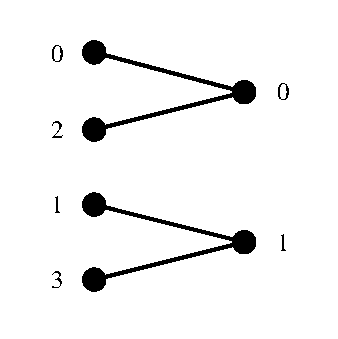
\includegraphics[scale=0.5]{Drawing1.pdf}
\caption{An example of a channel for which pseudo-group codes strictly outperform group codes. }
\label{fig: examp channel}
\end{figure}

Finally having Lemma \ref{lem: pseudo_group_for_chann_Z_4} and \ref{lem: group_chann_z_4}, there is a channel $(\mathcal{X}=\ZZ_4,\mathcal{Y}, W_{Y|X})$ such that the achievable rate of pseudo-group codes is strictly greater than the capacity of group codes. To see this, consider channel given in  Fig. \ref{fig: examp channel}. For this channel $I(X;Y|[X])=0$ and $I(X;Y)=1$. Thus, the capacity of group codes for this channel is $I_{c.c}(X;Y)=0$ while that of the pseudo-group codes is $I(X;Y)=1$.

 
\section{The Source Coding Problem}
In this section we show that the ensemble of pseudo-group codes achieves the symmetric rate-distortion function of any discrete memoryless source $(\mathcal{X}, \mathcal{Z}=\ZZ_{p^r}, P_X,d)$. in addition, it is shown that in some cases pseudo-group codes strictly outperform group codes.

The problem of source coding using group codes is studied in [Aria ?]. For a group $\ZZ_{p^r}$ and any integer $1\leq s \leq r$ define $\mathbf{H}_s=p^s\ZZ_{p^r}$. The following theorem derives an achievable rate for group codes: 


\begin{thm}\label{thm: group_codes_source}
Suppose $Z$ is a uniform random variable over $\ZZ_{p^r}$ with conditional distribution $P_{Z|X}$. Let $(\mathcal{X},\mathcal{Z}=\ZZ_{p^r},P_X,d)$ be a discrete-time and memoreless source. For a given distortion $D$, the achievable rate of group codes is 

\begin{equation*}
R_{g.s.c}(D) \geq \min_{P_{Z|X}: \EE\{d(Z,X\}\leq D }\max_{s=1}^r \frac{r}{s} I([Z]_s;X) 
\end{equation*}

where $[Z]_s=Z+\mathbf{H}_s$.

\end{thm}



%%%\begin{thm}
%%%Let $(\mathcal{X},\mathcal{Z},P_X,d)$ be a discrete-time and memoreless source. For a given distortion $D$, the achievable rate of group codes is 
%%%
%%%\begin{equation*}
%%%R(D)=\inf_{\alpha, \omega} \inf_{Z} \max_{\hat{\theta}\neq 0} \frac{1}{\omega_{\hat{\theta}}}\sum_{\eta, b}\alpha_{\eta,b} I([Z_{\eta,b}]_{\hat{\theta}};X)
%%%\end{equation*}
%%%where $\alpha, \omega$ and $U$ need to satisfy
%%%
%%%\begin{equation*}
%%%\sum_{\eta, b} \alpha_{\eta, b} \EE\{d(X,U_{\eta, b}\}\leq D
%%%\end{equation*}
%%%\end{thm}

Consider the ensemble of pseudo-group codes defined in Section \ref{sec: pseudo+group}. We use this ensemble to achieve the symmetric rate-distortion function:
\begin{thm}\label{thm: source coding pseudo group codes}
The ensemble of pseudo-group codes achieves the symmetric rate-distortion function for the source $(\mathcal{X},\mathcal{Z}=\ZZ_{p^r},P_X,d)$.
\end{thm}

The next subsection provides the results for the especial case when the underlying group is $\ZZ_4$. Also, theorem \ref{thm: source coding pseudo group codes} is proved for this special case.


\subsection{Results for $\ZZ_4$}
In this subsection we first prove theorem \ref{thm: source coding pseudo group codes} for the special case when $\mathcal{Z}=\ZZ_4$. Then we show that pseudo-group codes strictly outperform group codes. 

Consider the source $(\mathcal{X},\mathcal{Z}=\ZZ_4,P_X,d)$. We show that pseudo-group codes achieve the symmetric rate-distortion function. Similar to the channel coding problem we use a random coding argument. A random code-book $\mathcal{C}$ is the image of a random map $\phi$ ( defined in (\ref{eq: phi})) that is shifted by a random vector $B^n \in \ZZ_4^n$. Let $D$ be a non-negative real number. Fix a joint distribution $P_{XZ}$ such that $\EE\{d(X,Z)\}\leq D$ and $P_{Z}$ as the marginal of $P_{XZ}$ is uniform over $\ZZ_4$.  Given a sequence $x^n$ of the source, the encoder finds $\mathbf{a}\in J$ such that $z^n=\phi(\mathbf{a})+B^n$ is jointly typical with $x^n$ with respect to the probability distribution $P_{XZ}$. If there are more than one such $\mathbf{a}$, randomly select one. An error is declared, if no such $\mathbf{a}$ is found.  Upon receiving the sequence $\mathbf{a}$, the decoder reveal $z^n$ as the source reconstruction.

Suppose there is no error in the encoder. Since $z^n$ is jointly typical with $x^n$, for large enough $n$, $\frac{1}{n}\sum _{i=1}^n d(x_i,z_i)\approx \EE\{d(X,Z)\}\leq D$. Therefore, it remains to find conditions so that the probability of encoding error goes to $0$.

For $x^n\in \mathcal{X}^n$, define
 \begin{equation*}
 \theta(x^n)=\sum_{z^n \in A_{\epsilon}^n(Z|x^n)}\mathbbm{1}\{z^n \in \mathcal{C}\}
 \end{equation*}

 We can write $\theta(x^n)$ as

\begin{equation*}
 \theta(x^n)=\sum_{z^n \in A_{\epsilon}^n(Z|x^n)}\sum_{\mathbf{a}\in J}\mathbbm{1}\{z^n = \phi(\mathbf{a})+B^n\}
\end{equation*}

Note $\theta(x^n)$ is the number of code-words in $\mathcal{C}$ that are jointly typical with $x^n$. Thus an encoding error occurs if and only if $\theta(x^n)=0$. We use the Chebyshev's inequality to bound the probability of $\theta(x^n)=0$:
\begin{equation*}
P(\theta(x^n)=0)\leq \frac{Var\{\theta(x^n)\}}{\EE\{\theta(x^n)\}^2}
\end{equation*}

We have

\begin{align*}
\EE\{\theta(x^n)\}&= \sum_{z^n \in A_{\epsilon}^n(Z|x^n)}\sum_{\mathbf{a}\in J}P\{z^n = \phi(\mathbf{a})+B^n\}\\
&=\frac{|A_{\epsilon}^n(Z|x^n)|\cdot |J|}{4^n}\\
&\approx \frac{|J|}{4^n}2^{nH(Z|X)}
\end{align*}


To calculate $Var\{\theta(x^n)\}$ first need to calculate
\begin{align*}
\EE\{\theta(x^n)^2\}&= \sum_{\tilde{z}^n, z^n \in A_{\epsilon}^n(Z|x^n)}\sum_{\tilde{\mathbf{a}}, \mathbf{a}\in J}P\{z^n = \phi(\mathbf{a})+B^n,\tilde{z}^n = \phi(\mathbf{\tilde{a}})+B^n\}\\
&= \sum_{z^n \in A_{\epsilon}^n(Z|x^n)}\sum_{\mathbf{a}\in J}P\{z^n = \phi(\mathbf{a})+B^n\}+\sum_{\tilde{z}^n \neq z^n \in A_{\epsilon}^n(Z|x^n)}\sum_{\tilde{\mathbf{a}} \neq \mathbf{a}\in J}P\{z^n = \phi(\mathbf{a})+B^n,\tilde{z}^n = \phi(\mathbf{\tilde{a}})+B^n\}
\end{align*}

Using the above calculation and Lemma \ref{lem: probability of phi} and \ref{lem: Subgroup_typicality}, we have

\begin{align*}
\EE\{\theta(x^n)^2\} &\leq \frac{|J|}{4^n}2^{nH(Z|X)} + \sum_{\substack{ \tilde{z}^n , z^n \in A_{\epsilon}^n(Z|x^n)\\ \tilde{z}^n-z^n \in (2\ZZ_4)^n}}\sum_{\substack{ \tilde{\mathbf{a}}, \mathbf{a} \in J \\ \tilde{\mathbf{a}}-\mathbf{a} \in (2\ZZ_4)^{k_0} \times \{0\}^{k_1}}} \frac{1}{4^n}\frac{1}{2^n}\\
&+\sum_{\substack{ \tilde{z}^n , z^n \in A_{\epsilon}^n(Z|x^n)\\ \tilde{z}^n-z^n \notin (2\ZZ_4)^n}}\sum_{\substack{ \tilde{\mathbf{a}}, \mathbf{a}\in J \\ \tilde{\mathbf{a}}-\mathbf{a} \notin (2\ZZ_4)^{k_0} \times \{0\}^{k_1}}} \frac{1}{4^n}\frac{1}{4^n}\\
&\leq \frac{|J|}{4^n}2^{nH(Z|X)}+2^{nH(Z|X,[Z])}2^{nH(Z|X)} \frac{2^{k_0} \cdot |J|}{4^n \cdot 2^n}+2^{2nH(Z|X)} \frac{|J|^2}{4^n \cdot 4^n}
\end{align*}

Thus 
\begin{align*}
Var\{\theta(x^n)\}&=\EE\{\theta(x^n)^2\}-\EE\{\theta(x^n)\}^2\\
&\leq \frac{|J|}{4^n}2^{nH(Z|X)}+2^{nH(Z|X,[Z])}2^{nH(Z|X)} \frac{2^{k_0} \cdot |J|}{4^n \cdot 2^n}
\end{align*}


As a result, since $|J|=2^{2k_0+k_1}$, we have:

\begin{align*}
P(\theta(x^n)=0)&\leq \frac{Var\{\theta(x^n)\}}{\EE\{\theta(x^n)\}^2}\\
&\leq  2^{n\big(2-\frac{2k_0+k_1}{n} -H(Z|X)\big)} +   2^{n\big(1-\frac{k_0+k_1}{n}+H(Z|X,[Z])-H(Z|X)\big)}
\end{align*}

Therefore, in order to get $P(\theta(x^n)=0)\rightarrow 0$, we require the exponent of the above terms to be negative. Therefore, given the fact that $H(Z|X,[Z])-H(Z|X)=H([Z]|X)$, the following bounds need to be satisfied:
\begin{align*}
\frac{2k_0+k_1}{n} &> 2-H(Z|X)\\
\frac{k_0+k_1}{n} &> 1-H([Z]|X)
\end{align*}

The rate of the pseudo-group code is defined as $R=\frac{2k_0+k_1}{n}$. Hence, by the Fourier-Motzkin elimination, we get
\begin{align*}
R &> I(X;Z)\\
R+\frac{k_1}{n} &> 2I([Z];X)
\end{align*}

Setting $\frac{k_1}{n}=2I([Z];X)-I(Z;X)$ and given the fact that $2I([Z];X)-I(Z;X)\leq 1$, the equality $ R=I(X;Z) $ is achievable. Consequently by minimizing over $P_{Z|X}$, the symmetric rate-distortion function is achievable:
\begin{equation*}
R=\min_{P_{Z|X}: \EE\{d(X,Z)\}\leq D} I(X;Z)
\end{equation*}

Where $P_Z$ ( marginal of $P_{XZ}$) needs to be uniform over $\ZZ_4$.

Now to compare this ensemble with group cods we need the rate-distortion function of group codes:

\begin{lem}\label{lem: source coding_ groups_Z_4}
The achievable rate given in Theorem \ref{thm: group_codes_source} is tight when the underlying group is $\ZZ_4$. Hence the rate-distortion function of group codes is
\begin{equation}
R(D)=\min_{P_{Z|X: \EE\{d(X,Z)\}}}\max \{2I([Z];X), I(Z;X)\}
\end{equation} 
where $Z$ is uniform over $\ZZ_4$ and $[Z]=Z+2\ZZ_4$.
\end{lem}

The above lemma is a special case for a more general result addressed in \cite{Aria-group}. Now by Lemma \ref{lem: source coding_ groups_Z_4} and Theorem \ref{thm: source coding pseudo group codes}, it is immediate that pseudo-group codes strictly outperform group codes in certain source coding problems.







\section{Problem Statement}
In this paper, we explore the loss-less reconstruction of a determined function of two distributed sources. Our problem consists of two distributed sources that are distributively encoded and sent via a  multiple access channel (MAC). The receiver encodes the channels out put aiming to reconstruct a determined function of the two sources. We first model a pair of distributed sources by the following definition.


\begin{definition}[Sources]
A pair of distributed sources is modeled by two random processes. Suppose $S_1, S_2$ are two possibly dependent pair of discrete time random processes, both taking value from the set $\mathcal{S}$. We denote the corresponding pair of sources by $(S_1,S_2, \mathcal{S})$. Also let $P_{S_1,S_2}$ be the joint probability distribution of $S_1$ and $S_2$. The set $\mathcal{S}$ forms a group in this paper and usually denoted by $\mathbf{H}$ where $\mathbf{H}$ is a group with $+$ as the group operation. 
\end{definition}

Now suppose $(S_1,S_2,\mathcal{S}=\mathbf{H})$ is a pair of distributed sources, where $\mathbf{H}$ is a group. $S_1$ and $S_2$ are encoded to $X_1$ and $X_2$ respectively. Then $X_1, X_2$ communicate with a central receiver that is interested to reconstruct $X_1+X_2$, where $+$ is the group operation. This problem is a special case of a general problem called computation over MAC. Fig. ??? depicts a diagram of such problem. We define the corresponding MAC channel, in the following way: 


\begin{definition}(MAC)\label{def: MAC}
Suppose $X_1$ and $X_2$ are two random variables taking value from $\mathcal{X}=\mathbf{H}$, where $\mathbf{H}$ is a group with operation $+$. The MAC channel in this paper is defined by the conditional probability 
\begin{equation*}
W_{Y|X_1+X_2}
\end{equation*}
where $Y$ is the channel's output with alphabet $\mathcal{Y}$. $X_1, X_2$ are the two terminals of the MAC channel. As a short hand, we write sometimes this conditional probability as $W$. We denote such MAC channel by $(\mathcal{X},\mathcal{Y},W)$. 
\end{definition}


\begin{definition}(Code for computation over MAC)\label{def: code for comp over mac}
For positive integers $n,k$ and $\delta \geq 0$, a $(k,n,\delta)$-code for the computation over MAC consists of encoders $f_i:\mathcal{S}^k \rightarrow \mathcal{X}^n$ for $i=1,2$ and the decoder function $g:\mathcal{Y}^n \rightarrow \mathcal{S}^k$, such that if $Y^n$ is the output of the channel with input $f_1(S_1^k), f_2(S_2^k)$ then 
\begin{equation*}
P\{ g(Y^n)\neq S^k_1+S^k_2\}\leq \delta
\end{equation*} 

Where the group addition is element wise.
\end{definition}



\begin{definition}(Achievable rate)
We say $R$ is achievable if for some positive integer $n$ and any $\delta>0$, there exist a $(Rn,n,\delta)$-code.  
\end{definition}

Note that since we are interested only to recover $S_1+S_2$, decoding $S_1$ or $S_2$ incorrectly is not damaging. 
 
\section{Computation Over MAC}
For positive integer $r$ and a prime $p$ consider the MAC channel $(\mathcal{X}=\ZZ_{p^r},\mathcal{Y},W)$ as defined in Definition \ref{def: MAC}. Various previously known results showed that using structured codes for multi-terminal problems such as computation over MAC is beneficial. [Aria???] and [dinesh??] studied the applications of group codes for computation over MAC. Using the ensemble of group codes one can achieve larger rates than the Shannon standard approach. However, these achievable rates are note proved to be optimal. We show in this paper that indeed the achievable rates of group codes is not optimal. We further propose a new framework based on the pseudo-group codes such that under certain circumstances it extends all the previously know achievable rates. Let first drive an achievable rate region for the ensemble of group codes:

\begin{figure}
\centering
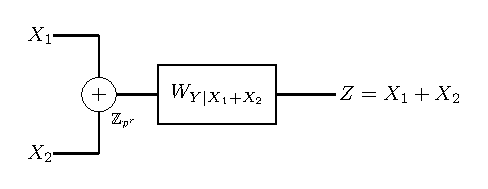
\includegraphics[scale=1]{Comp_Over_MAC.pdf} 
\caption{sds}
\end{figure}



\begin{thm}
For the $(\mathcal{X}=\ZZ_{p^r},\mathcal{Y},W)$, the ensemble of group codes achieves the following bound:

\begin{equation*}
R_{g,mac} \leq \min_{s=0}^{r-1} \frac{r}{r-s} I(X;Y|[X]_{s})
\end{equation*}
Where $X$ is assumed to be uniform over $\ZZ_{p^r}$.
\end{thm}


\begin{proof}
The proof is straightforward. For each of the two terminal use the same encoding scheme. Since the group is closed under it's operation having Theorem \ref{thm: group codes channel} proves the achievable rates in this case.
\end{proof}


\subsection{Pseudo-group codes for computation over MAC}
We propose a new framework based on the ensemble of pseudo-group codes. The framework involves an inner and an outer code. We first describe the inner code. The outer code will be addressed shortly. 

Similar to the pint-to-point setting, for a given positive integer $n$, a pseudo-group framework with length $n$ over the underlying group $\ZZ_{p^r}$ consists of $r$ layers of cods. For $i \in \{0,1,\cdots,r-1\}$, the $i^{th}$ layer has the generator matrix $\mathbf{G}_i$ of dimension $k_i\times n$ with elements belonging to $\ZZ_{p^r}$. Therefore, we can define the corresponding code-book of such framework as 

\paragraph*{Code-book}
Define the code-book of the $i^{th}$ layer as: 

\begin{equation}\label{eq: Pseudo_MAC layer i}
\mathcal{E}_i=\{ u_i^{k_i}\mathbf{G}_i: u_i^{k_i}\in T_i^{k_i}\}
\end{equation}
Where $T_i=\{0,1,\cdots, p^{r-i}-1\}$. Now the pseuso-group code is defined as:
\begin{equation}\label{eq: Pseudo_MAC codebook}
\mathcal{E}=\sum_{i=0}^{r-1} \mathcal{E}_i+b^n
\end{equation}

Where the summation is element-wise and $b^n\in \ZZ_{p^r}^n$ is a dither vector.  In contrary to the point-to-point setting, we use a specific binning strategy for $\mathcal{E}$ for the computation over MAC. We discuss about such binning later on this Section.
%Note the code-book $\mathcal{E}$ is differ from $\mathcal{C}$ defined for point-to-point communications. For $\mathcal{C}$, elements of $u_i^{k_i}$ belong to the subset $T_i$ while in $\mathcal{E}$ it belongs to the whole group $\ZZ_{p^r}$. Therefore, $\mathcal{E}$ is a larger code-book than $\mathcal{C}$.
To define the coding scheme, it is required by Definition \ref{def: code for comp over mac} to define two encoding functions and one decoding rule. The binning strategy is proposed in the definition of the error event.

\paragraph*{Encoders}

Since there are $r$ distinct layers of coding the message is supposed to belong to 

\begin{equation*}
\mathcal{J}=\bigoplus_{i=0}^{r-1} T_i^{k_i}
\end{equation*}

 Define the map 
\begin{align}\label{eq: phi_mac}
&\Phi :\mathcal{J} \rightarrow \ZZ_{p^r}^n\\\nonumber
& \Phi(\mathbf{a}):=\sum_{i=0}^{r-1} u_i^{k_i}\mathbf{G}_i 
\end{align}

where $\mathbf{s}=(u_0^{k_0},u_0^{k_1}, \cdots, u_{r-1}^{k_{r-1}})$ is an element of $\mathcal{J}$. Choose two distinct vectors $b_1^n$ and $b_2^n$ with elements belonging to $\ZZ_{p^r}$. Define the encodes function by 
\begin{equation*}
f_i(\mathbf{s}_1)=\Phi(\mathbf{s}_i)+b_i^n \quad  for \quad  i=1,2
\end{equation*}

\paragraph*{Decoder}
Upon receiving $y^n$, the channel's output, the decoder finds $\mathbf{z} \in \mathcal{J}+\mathcal{J}$ (with the element wise addition) such that $\Phi(\mathbf{z})+b_1^n+b_2^n$ is jointly typical with $y^n$ with respect to the distribution $P_Z \cdot W_{Y|X_1+X_2}$ where $P_Z$ is a uniform distribution over $\ZZ_{p^r}$. 

\paragraph*{Error Event}
 The error is declared in if of the two event $E_1$ or $E_2$ occurs.  Let $\mathbf{z}=\mathbf{a}_1+\mathbf{a}_2$. $E_1$ occurs if there is no $\mathbf{z} \in \mathbf{J}$ such that $\Phi(\mathbf{z})+b_1^n+b_2^n$ is jointly typical with $y^n$. To define the event $E_2$, let first define a few terms. For integer $i=0,1$, define the subgroup $\mathbf{H}_i=p^{r-i} \ZZ_{p^r}$. Note $T_i$ is a transversal for the subgroup $\mathbf{H}_i$ in $\ZZ_{p^r}$. Therefore, given $i$, any element $g$ in $\ZZ_{p^r}$ can be written as $g=t_i+h_i$ for a $t_i \in T_i$ and some $h_i \in \mathbf{H}_i$. Now $\forall g \in \ZZ_{p^r}$ define $[g]_i=t_i$ where $i$ ranges from $0$ to $r-1$. Consequently, $[\cdot]_i$ can be regarded as a well defined map from $\ZZ_{p^r}$ to $T_i$. Suppose $\mathcal{S}=\bigoplus_{i=0}^{r-1} \ZZ_{p^r}^{k_i}$. For the special case where $i=0$, it gives $[g]_0=g$. Now define the map 

\begin{align*}
&\pi : \mathcal{S} \rightarrow \mathcal{J}\\
&\pi(\mathbf{s})=\big ( [u_i^{k_i}]_i \big )_{i=0}^{r-1}
\end{align*}

where $[\cdot ]_i$ are applied element wise.

Now we are ready to define the second error event. $E_2$ occurs if there is another sequence $\tilde{\mathbf{z}}$ jointly typical with $y^n$ such that

\begin{equation*}
\pi(\mathbf{z}-\tilde{\mathbf{z}}) \neq \mathbf{0}
\end{equation*}

Note if $u_i^{k_i}-\tilde{u}_i^{k_i} \in \mathbf{H}_i^{k_i}$ then no error is declared. Intuitively such definition for the error event is to construct a central binning strategy for each layer of the code. In this strategy, for $i^{th}$ layer, two code-words $u_i^{k_i}\mathbf{G}_i$ and $\tilde{u}_i^{k_i}\mathbf{G}_i$ belong to the same bin, if $u_i^{k_i}$ and  $\tilde{u}_i^{k_i}$ belong to the same co-set of the subgroup $\mathbf{H}^{k_i}_i$ in the group $\ZZ^{k_i}_{p^r}$. Consequently, each bin for the total code is the image of the corresponding co-set of the subgroup $$\bigotimes_{i=0}^{r-1} \mathbf{H}_i^{k_i}$$ under the map $\Phi(\cdot)$.

\paragraph*{Rate of the code}
The rate of this code is  
\begin{equation}
R=\frac{1}{n} \log_2 |\mathcal{E}|= \sum_{i=0}^{r-1} \frac{k_i}{n} \log_2 |T_i| = \sum_{i=0}^{r-1} \frac{k_i}{n} (r-i) \log_2 p
\end{equation}



The outer code applied to all layers of codes except the first layer. Thus, it consists of $r-1$ layers of codes. Now given the binning strategy and the inner code the $i^{th}$ layer of the outer code corresponding to $i^{th}$ layer of the inner code sees a MAC channel depicted in Fig. \ref{fig: outer mac}. In this figure $[\cdot ]_i$ is as defined in the Error Event paragraph. Fig. \ref{fig: outer mac} is a noiseless computation over MAC in which the receiver wants to reconstruct  $X_1+X_2$ where the summation is the $\ZZ_{p^r}$ group addition. The symmetric capacity of this channel is achievable using standard structured codes such as \textit{Nested Polar Codes}, \cite{Aria-polar}. The following lemma drives the symmetric capacity of the computation over MAC shown in Fig. \ref{fig: outer mac}.


\begin{lem}\label{lem: outer_mac_capacity}
The capacity of the channel in Fig. \ref{fig: outer mac} is 
\begin{equation*}
C_i=(r-i) \log_2 p - H(S_1+S_2|[S_1+S_2]_i)
\end{equation*}

where the addition is the group $\ZZ_{p^r}$ operation and $S_1, S_2$ are uniform random variable taking values from $\ZZ_{p^r}$ .
\end{lem} 

Having Lemma \ref{lem: outer_mac_capacity}, one can conclude that the achievable rate of the outer code for $i^{th}$ layer is $C_i$. Define the normalized capacity of this channel as 

\begin{equation*}
\alpha_i =\frac{C_i}{(r-i) \log_2 p}
\end{equation*}

Noe the effective rate of the framework is 

\begin{equation*}
R= \sum_{i=0}^{r-1} \frac{k_i}{n}  \alpha_i (r-i) \log_2 p
\end{equation*}




\begin{figure}
\centering
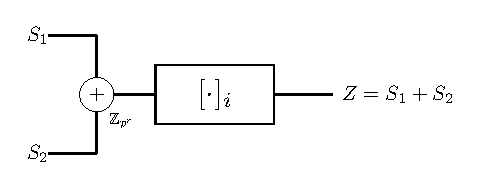
\includegraphics[scale=1]{sss.pdf} 
%\input{sss.tex}
\caption{The outer MAC channel. }
\label{fig: outer mac}
\end{figure}







For fixed $n$ and $k_i$, the random ensemble of pseudo-group codes consists of all codes of the form $\mathcal{E}$ where elements of the generator matrices $\mathbf{G}_i$ and dither vector $b^n$ are chosen independently of each other and uniformly from the set $\ZZ_{p^r}$. Using a random coding argument we can 



\begin{thm}
The achievable rate of pseudo-group codes for the MAC channel $(\mathcal{X},\mathcal{Y}, P_{Y|X_1+X_2})$ is

\begin{equation*}
R \leq \sum_{s=0}^{r-1} \alpha_s |\min_{s+1\leq i\leq r} I_{[p^i]}-I_{p^{s}}|
\end{equation*}
\end{thm}













\section{Group Codes with $\{ 0,1\}$ generator matrices}\label{sec: group codes with 0,1 gen mtx}
In this draft, we will show that the ensemble of uniform random group codes in $\ZZ_4$ with $\{ 0,1\}$-generator matrices followed by a group code with rate approaching to 2, can achieve the following rate region over any discrete memoryless channel with input $\ZZ_4$:

\begin{align*}
R&<2-H(X|Y)\\
R&< 2-H(X|Y,[X]_{\{ 0,2\}})
\end{align*}

where $[X]_{\{ 0,2\}}$ denotes the mapping from $\ZZ_4$ to $\ZZ_4/2\ZZ_4$ with $x\rightarrow x+2\ZZ_4$. 

Moreover, we propose a more general construction of such group codes by adding an extra component. We show that using the proposed construction we can achieve a larger rate region. 

\begin{definition}
Suppose $\mathcal{X}=\{\alpha_1,\alpha_2,\cdots, \alpha_N \}$ where $N$ is a positive integer and $\alpha_i$'s are distinct. For a sequence $x^n\in \mathcal{X}^n$ define it's n-type as $t_n(x^n):=(t(x^n,\alpha_1),t(x^n,\alpha_2),\cdots, t(x^n,\alpha_N))$ where $t(x^n,\alpha_i):= \frac{1}{n} |\{ j: x_j=\alpha_i\}|$. Let $\mathcal{T}_n(\mathcal{X})$ be the set of all n-types on $\mathcal{X}$. Also, let $\mathcal{P}(X)$ denotes the set of all probability distributions on $\mathcal{X}$. For $V\in \mathcal{T}_n(\mathcal{X})$, define $T_{\mathcal{X}}^n(V):=\{ x^n\in \mathcal{X}^n|t(x^n)=V\}$.
\end{definition}

\begin{definition}
For random variable $X$ taking values in $\mathcal{X}$ and  $\epsilon>0$, define $A_\epsilon^n(X)$ the set of all typical sequences with length $n$. If $P_X$ is the probability distribution of $X$, for $\delta>0$, define: 

\begin{equation*}
\mathcal{T}_\delta^n(X):=\{ V_X\in \mathcal{T}_n(\mathcal{X}) : ~ \|V_X(x)-P_X(x)\|<\delta, \forall x\in \mathcal{X}\} 
\end{equation*}

Similarly, for a pair of random variables $X,Y$,  define $\mathcal{T}_\delta^n(X,Y)$ and $\mathcal{T}_\delta^n(X|Y)$. 
\end{definition}

\begin{definition}
For a matrix $\mathbf{G}\in \{0,1\}^{k \times n}$ and a vector $b^n\in \ZZ_4^n$ define  
\begin{equation}
\mathcal{C}:=\{ u^k\mathbf{G}+b^n|u^k\in \ZZ_4^k\}
\end{equation}

Note $\mathcal{C}$ represents the codebook of the group code over $\ZZ_4$ generated by $\mathbf{G}$ with dither $b^n$. 
\end{definition}

Let $(\mathcal{X},\mathcal{Y}, W)$ denote a discrete memoryless channel with input alphabet $\mathcal{X}$, output alphabet $\mathcal{Y}$ and conditional probability distribution $W \in \mathcal{P}(X|\mathcal{Y})$. 

Given message $u^k$ the encoder sends $u^k\mathbf{G}+b^n$. The decoding can be performed by typicality decoding. Upon receiving the channel's output sequence $y^n$ the decoder declares error if there is no code word in $\mathcal{C}$ which is jointly typical with $y^n$ or if there are more than one of such codewords. 

Suppose that the message sequences $u^k$ are chosen  equally likely. Thus for a fixed $\mathbf{G}$ and $b^n$ the average error probability of $\mathcal{C}$ for channel $(\mathcal{X}=\ZZ_4, \mathcal{Y},W)$ is

\begin{align*}
P_{err}(\mathbf{G},b^n):=\sum_{u^k\in \ZZ_4^k}\frac{1}{4^k} \sum_{x^n\in A_\epsilon^n(X)} \mathbbm{1}\{ u^k \mathbf{G}+b^n=x^n\} \sum_{y^n\in A_\epsilon^n(Y|x^n)}  W^n(y^n|x^n) \mathbbm{1}\{ \exists ~ \tilde{x}^n\in \mathcal{C} \cap A_\epsilon^n(X|y^n), \tilde{x}^n\neq x^n \}
\end{align*}

Note
\begin{align*}
\mathbbm{1}\{ \exists ~ \tilde{x}^n\in \mathcal{C} \cap A_\epsilon^n(X|y^n), \tilde{x}^n\neq x^n \}=\sum_{\substack{\tilde{u}^k \in \ZZ_4^k \\\tilde{u}^k\neq u^k}}\sum_{\tilde{x}^n\in A_\epsilon^n(X|y^n)}\mathbbm{1}\{ \tilde{u}^k\mathbf{G}+b^n=\tilde{x}^n\}
\end{align*}

Now consider the ensemble of all group codes with generator matrix $\mathbf{G}$ of size $k \times n$ and dither $b^n$. Suppose elements of $\mathbf{G}$  are independently and uniformly chosen from the set $\{ 0,1\}$. Also let $b_i$'s be chosen randomly, independent of $\mathbf{G}$ with uniform distribution over $\ZZ_4$. Then the average error probability over all such codes is
.
\begin{align}\label{equ: p_err}
P_{err}&=\EE\{ P_{err}(\mathbf{G},b^n) \}\\
&=\sum_{u^k\in \ZZ_4^k} \sum_{\substack{\tilde{u}^k \in \ZZ_4^k \\\tilde{u}^k\neq u^k}} \sum_{x^n\in A_\epsilon^n(X)} \sum_{y^n\in A_\epsilon^n(Y|x^n)} \sum_{\tilde{x}^n\in A_\epsilon^n(X|y^n)} \frac{1}{4^k} W^n(y^n|x^n) \PP\{ \tilde{u}^k\mathbf{G}+b^n=\tilde{x}^n, u^k \mathbf{G}+b^n=x^n\} 
\end{align}


Since $b^n$ is uniform over $\ZZ_4^n$ then 

\begin{align} \label{equ: p_u}
\PP\{ \tilde{u}^k\mathbf{G}+b^n=\tilde{x}^n, u^k \mathbf{G}+b^n=x^n\}=\frac{1}{4^n}\PP\{ (\tilde{u}^k-u^k)\mathbf{G}=(\tilde{x}^n-x^n)\}
\end{align}

Assume $t_k(\tilde{u}^k-u^k)=q$. Depending on $q$ there are three cases for  $\PP\{ (\tilde{u}^k-u^k)\mathbf{G}=(\tilde{x}^n-x^n)\}$:

\begin{enumerate}
\item[Case 1:] $q(1)+q(3)=0$ i.e., $(\tilde{u}^k-u^k)\in 2\ZZ_4^k$.
\item[Case 2:] $q(1)+q(3)>0, q(2)>0$.
\item[Case 3:] $q(1)+q(3)>0, q(2)=0$.
\end{enumerate}

 The following lemma considers Case 1 and 2. 
\begin{lem}\label{lem: p_u}
 If $u^k \in \ZZ_4^k, x^n\in \ZZ_4^n$ are two none zero sequences then the following hold for  $P:=\PP\{ u^k\mathbf{G}=x^n\}$
\begin{enumerate}
\item If $u^k\in 2 \ZZ_4^k$ then $P=\frac{1}{2^n}$ for $x^n \in 2 \ZZ_4^n$ otherwise $P=0$.
\item If  $u^k \notin 2 \ZZ_4^k$,  $t_k(u^k, 2)>0$ then  $P=\frac{1}{4^n}$.
\end{enumerate}
\end{lem}

\begin{proof}
For the first statement note that if $u^k\in 2 \ZZ_4^k$ then $ u^k\mathbf{G}\in 2 \ZZ_4^k$. Thus $P=0$ when $x^n \notin 2 \ZZ_4^n$. As $u^k\in 2\ZZ_4^k-0^k$,without loss of generality assume $u_1=2$. Therefore, $P$ can be written as $\PP\{ 2\mathbf{G}_1=x^n-\sum_{i>1} u_i \mathbf{G}_i\}$ where $\mathbf{G}_i$ is the $i^{th}$ row of $\mathbf{G}$. Hence in this case, $P=\frac{1}{2^n}$


The proof for 2. is similar. Since $u^k \notin 2 \ZZ_4^k$ and $t(u^k, 2)>0$, there exist two indices $i,i'$ with $u_{i}=2$ and $u_{i'}=1$ or $3$. Without loss of generality let $i=1, i'=2$. It can be shown that $2\mathbf{G}_1+\mathbf{G}_2$ and $2\mathbf{G}_1+3\mathbf{G}_2$ are uniform over $\ZZ_4^n$. Thus if $u_2=1$,  $P=\PP\{ 2\mathbf{G}_1+\mathbf{G}_2=x^n-\sum_{i>2} u_i \mathbf{G}_i\}=\frac{1}{4^n}$. The same result holds if $u_2=3$.
\end{proof}

For the third case we need another lemma.

\begin{lem}\label{lem: p_u case 3}
Suppose $Z^n=u^k\mathbf{G}$; where elements of $\mathbf{G}$ are chosen randomly, uniformly and independently of each other from $\{ 0,1 \}$.  Then $Z_i$ are i.i.d and if $t_k(u^k)=q, t_n(x^n)=r$ then
\begin{equation}
\PP\{ Z^n=x^n\}=2^{-nD(r\| Q_{k,q})-nH(r)}
\end{equation}
where $Q_{k,q}$ is the distribution of $Z_i$. Moreover $Q_{k,q}$ depends on $u^k$ only through its type.
\end{lem}

\begin{proof}
Since elements of $\mathbf{G}$ are independent, $Z_i$'s are also independent. By definition $Z_i=\sum_{j=1}^{k} u_j\mathbf{G}_{ji}$. For $z\in \ZZ_4$, let $I_z:=\{l: u_l=z\}$. Then, $Z_i=\sum_{z=\ZZ_4} \sum_{l\in I_z} z\mathbf{G}_{li}$.  Hence, as $\mathbf{G}_{li}$'s have identical distributions, $Z_i$'s also have identical distributions. Thus, $Z_i$'s are i.i.d. For simplicity, let $Z$ denote any of such $Z_i$'s. The distribution of $Z$ only depends on the size of $I_z$'s. Since $|I_z|=kq(z)$, we can denote the distribution of $Z$ by $Q_{k,q}$, i.e., $\PP\{Z_i=x\}=\PP\{Z=x\}:=Q_{k,q}(x)$ for $x\in \ZZ_4$. Therefore, given the type of $x^n$, we have
\begin{align*}
\PP\{ Z^n=x^n\}&=\prod_{z\in \ZZ_4}\PP\{ Z=z\}^{nr(z)}\\
&=\prod_{z\in \ZZ_4}Q_{k,r}(z)^{nr(z)}\\
&=2^{n\sum_{z\in \ZZ_4}{r(z)\log_2(Q_{k,r}(z))} }
\end{align*}

Note that

\begin{align*}
\sum_{z\in \ZZ_4}{r(z)\log_2(Q_{k,r}(z))}&=\sum_{z\in \ZZ_4}{r(z)\log_2(\frac{Q_{k,r}(z)}{r(z)})}+\sum_{z\in \ZZ_4}{r(z)\log_2(r(z))}\\
&=-D(r\| Q_{k,q})-H(r)
\end{align*}
This completes the proof.
\end{proof}


Let $S_q:=\{q\in \mathcal{T}_k(\ZZ_4) | q(1)+q(3)>0, q(2)>0 \}$ and $\tilde{S}_q:=\{q\in \mathcal{T}_k(\ZZ_4) | q(1)+q(3)>0, q(2)=0 \}$.  (\ref{equ: p_err}) is divided into three terms: 
\begin{align} \label{equ: p_err_1}\nonumber
P_{err}&=
\sum_{\substack{u^k, \tilde{u}^k \in \ZZ_4^k \\ (\tilde{u}^k-u^k)\in 2\ZZ_4^k}} \sum_{x^n\in A_\epsilon^n(X)} \sum_{y^n\in A_\epsilon^n(Y|x^n)} \sum_{\substack{\tilde{x}^n\in A_\epsilon^n(X|y^n)} } \frac{1}{4^k}\frac{1}{4^n} W^n(y^n|x^n)\PP\{ (\tilde{u}^k-u^k)\mathbf{G}=(\tilde{x}^n-x^n)\}\\\nonumber
%
&+\sum_{q\in S_q}\sum_{\substack{u^k, \tilde{u}^k \in \ZZ_4^k \\ t(\tilde{u}^k-u^k)=q}} \sum_{x^n\in A_\epsilon^n(X)} \sum_{y^n\in A_\epsilon^n(Y|x^n)} \sum_{\substack{\tilde{x}^n \in A_\epsilon^n(X|y^n)} } \frac{1}{4^k}\frac{1}{4^n}  W^n(y^n|x^n) \PP\{ (\tilde{u}^k-u^k)\mathbf{G}=(\tilde{x}^n-x^n)\}\\
%
&+\sum_{q\in \tilde{S}_q}\sum_{\substack{u^k, \tilde{u}^k \in \ZZ_4^k \\ t(\tilde{u}^k-u^k)=q}} \sum_{r\in\mathcal{T}_n(\mathcal{X}) } \sum_{x^n\in A_\epsilon^n(X)} \sum_{y^n\in A_\epsilon^n(Y|x^n)} \sum_{\substack{\tilde{x}^n\in A_\epsilon^n(X|y^n)\\t(\tilde{x}^n-x^n)=r} } \frac{1}{4^k}\frac{1}{4^n} W^n(y^n|x^n)\PP\{ (\tilde{u}^k-u^k)\mathbf{G}=(\tilde{x}^n-x^n)\}
\end{align}


Applying  lemma \ref{lem: p_u} for the first two terms of (\ref{equ: p_err_1}) and lemma \ref{lem: p_u case 3} for the third term yield: 
\begin{align}\label{p_err_part 1}
P_{err}&=
\sum_{\substack{u^k, \tilde{u}^k \in \ZZ_4^k \\ (\tilde{u}^k-u^k)\in 2\ZZ_4^k}} \sum_{x^n\in A_\epsilon^n(X)} \sum_{y^n\in A_\epsilon^n(Y|x^n)} \sum_{\substack{\tilde{x}^n\in A_\epsilon^n(X|y^n)\\(\tilde{x}^n-x^n)\in 2\ZZ_4^n} } \frac{1}{4^k}\frac{1}{4^n} \frac{1}{2^n} W^n(y^n|x^n)\\\label{p_err_part 2}
%
&+\sum_{q\in S_q}\sum_{\substack{u^k, \tilde{u}^k \in \ZZ_4^k \\ t(\tilde{u}^k-u^k)=q}} \sum_{x^n\in A_\epsilon^n(X)} \sum_{y^n\in A_\epsilon^n(Y|x^n)} \sum_{\substack{\tilde{x}^n \in A_\epsilon^n(X|y^n)} } \frac{1}{4^k}\frac{1}{4^n} \frac{1}{4^n} W^n(y^n|x^n)\\\label{p_err_part 3}
%
&+\sum_{q\in \tilde{S}_q}\sum_{\substack{u^k, \tilde{u}^k \in \ZZ_4^k \\ t_k(\tilde{u}^k-u^k)=q}} \sum_{r\in\mathcal{T}_n(\mathcal{X}) } \sum_{x^n\in A_\epsilon^n(X)} \sum_{y^n\in A_\epsilon^n(Y|x^n)} \sum_{\substack{\tilde{x}^n\in A_\epsilon^n(X|y^n)\\t_n(\tilde{x}^n-x^n)=r} } \frac{1}{4^k}\frac{1}{4^n} W^n(y^n|x^n)2^{-nD(r\| Q_{k,q})-nH(r)}
\end{align}


Define the rate of the code as $R=\frac{2k}{n}$.
\begin{lem} \label{lem: part 1&2}
(\ref{p_err_part 1}) and (\ref{p_err_part 2}) converge to $0$ if 
\begin{align*}
R&<2-H(X|Y)\\
R&<2-H(X|Y,[X]_{\{ 0,2\}})
\end{align*}
\end{lem}


\begin{proof}
The proof is straightforward. 
\end{proof}

Denote the third term in $P_{err}$, i.e., (\ref{p_err_part 3}),  by $P_{err,3}$. Having Lemma \ref{lem: part 1&2}, it remains to find the necessary conditions on $R$ to let $P_{err,3}$ converge to zero. By Lemma \ref{lem: p_u case 3}, since the inner terms of the sums in $P_{err,3}$ depend on $u^k, \tilde{u}^k$ only through type $q$, we can replace the summation over $u^k, \tilde{u}^k$ by $|\{ (u^k, \tilde{u}^k):t(\tilde{u}^k-u^k)=q \}|=4^k 2^{kH(q)}$. Therefore, we have:

\begin{align*}
P_{err,3}=\sum_{q\in \tilde{S}_q}\sum_{r\in\mathcal{T}_n(\mathcal{X}) } \sum_{x^n\in A_\epsilon^n(X)} \sum_{y^n\in A_\epsilon^n(Y|x^n)} \sum_{\substack{\tilde{x}^n\in A_\epsilon^n(X|y^n)\\t_n(\tilde{x}^n-x^n)=r} } \frac{1}{4^n} W^n(y^n|x^n)2^{-nD(r\| Q_{k,q})-nH(r)+kH(q)}
\end{align*} 

Summations over $x^n, y^n$ and $\tilde{x}^n$ can be replaced by  two summations; one on a set of joint types over $(\mathcal{X}\times \mathcal{Y})$ and $(\tilde{\mathcal{X}} \times \mathcal{Y})$ and the other over triples $(x^n, y^n, \tilde{x}^n)$ in the following manner:


\begin{lem}\label{lem: p_err3, F_n}
For joint types $V_{XY}\in \mathcal{T}_n(\mathcal{X}\times \mathcal{Y}), W_{\tilde{X}Y} \in \mathcal{T}_n(\tilde{\mathcal{X}}\times \mathcal{Y}) $ and $r\in \mathcal{T}_n(\mathcal{X})$, define:
\begin{equation*}
F_n(V_{XY},W_{\tilde{X}Y},r):=\{(x^n,y^n,\tilde{x}^n): t_n(x^n,y^n)=V_{XY}, t_n(\tilde{x}^n,y^n)=W_{XY}, t_n(\tilde{x}^n-x^n)=r \}
\end{equation*}

Then $P_{err,3}$ can be written as:

\begin{align} \label{equ: p_err3, F_n}
P_{err,3}=\sum_{q\in \tilde{S}_q}\sum_{r\in\mathcal{T}_n(\mathcal{X}) } \sum_{\substack{V_{XY}\in \mathcal{T}_\epsilon^n(X,Y)\\ W_{\tilde{X}Y}\in  \mathcal{T}_\epsilon^n(\tilde{X},Y) }} \sum_{(x^n,y^n,\tilde{x}^n)\in F_n(V_{XY},W_{\tilde{X}Y},r)}  \frac{1}{4^n} W^n(y^n|x^n)2^{-nD(r\| Q_{k,q})-nH(r)+kH(q)}
\end{align}

\end{lem}
\begin{proof}
$P_{err,3}$ can be written as

\begin{align*}
P_{err,3}=\sum_{q\in \tilde{S}_q}\sum_{r\in\mathcal{T}_n(\mathcal{X}) } \sum_{(x^n,y^n,\tilde{x}^n)\in B_\epsilon^n(X,Y,\tilde{X},r)}  \frac{1}{4^n} W^n(y^n|x^n)2^{-nD(r\| Q_{k,q})-nH(r)+kH(q)}
\end{align*}

where
\begin{align*}
B_\epsilon^n(X,Y,\tilde{X},r):=\{ (x^n,y^n,\tilde{x}^n)| (x^n,y^n)\in A_\epsilon^n(X,Y),(\tilde{x}^n,y^n)\in A_\epsilon^n(\tilde{X},Y),  t_n(\tilde{x}^n-x^n)=r \}
\end{align*}



 Summation over triple $(x^n,y^n,\tilde{x}^n)$ can be divided into two summations as follows:

\begin{align*}
P_{err,3}=\sum_{q\in \tilde{S}_q}\sum_{r\in\mathcal{T}_n(\mathcal{X}) } \sum_{\substack{V_{XY}\in \mathcal{T}_\epsilon^n(X,Y)\\ W_{\tilde{X}|Y}\in  \mathcal{T}_\epsilon^n(\tilde{X}|Y) }} \sum_{(x^n,y^n,\tilde{x}^n)\in G_n(V_{XY},W_{\tilde{X}|Y},r)}  \frac{1}{4^n} W^n(y^n|x^n)2^{-nD(r\| Q_{k,q})-nH(r)+kH(q)}
\end{align*}

where

\begin{equation*}
G_n(V_{XY},W_{\tilde{X}|Y},r):=\{(x^n,y^n,\tilde{x}^n): t_n(x^n,y^n)=V_{XY}, t_n(\tilde{x}^n|y^n)=W_{\tilde{X}|Y}, t_n(\tilde{x}^n-x^n)=r \}
\end{equation*}

Suppose that the conditional type induced by $W_{\tilde{X}Y}$ is $W_{\tilde{X}|Y}$. Let $V_Y, W_Y$ be the marginal types of $V_{XY}$ and $W_{\tilde{X}Y}$, respectively. If $V_Y \neq W_Y$ then, $F_n(V_{XY},W_{\tilde{X}Y},r)=\emptyset$; otherwise, $F_n(V_{XY},W_{\tilde{X}Y},r)=G_n(V_{XY},W_{\tilde{X}|Y},r)$. Therefore, $P_{err,3}$ can be written as in (\ref{equ: p_err3, F_n}) and the proof is complete.
\end{proof}


For joint types $V_{XY},W_{\tilde{X}Y}$ and type $r$, define:
\begin{equation*}
S_n(V_{XY},W_{\tilde{X}Y},r):=\{ U_{XY\tilde{X}} \in \mathcal{T}_n(\mathcal{X},\mathcal{Y},\tilde{\mathcal{X}})| U_{XY}=V_{XY}, U_{\tilde{X}Y}=W_{\tilde{X}Y}, U_{\tilde{X}-X}=r\}
\end{equation*}

\begin{lem}\label{lem: F_n}
 The following bound on the size of $F_n(V_{XY},W_{\tilde{X}Y},r)$ holds:

\begin{align*}
| F_n(V_{XY},W_{\tilde{X}Y},r) | \leq 2^{nH_{s,n}(V_{XY},W_{\tilde{X}Y},r)+O(\log n)}
\end{align*}

where

\begin{equation*}
H_{s,n}(V_{XY},W_{\tilde{X}Y},r):= \max_{a\in S_n(V_{XY},W_{\tilde{X}Y},r)} H(a)
\end{equation*}
\end{lem}

\begin{proof}
\begin{equation*}
| F_n(V_{XY},W_{\tilde{X}Y},r) | =\sum_{a\in S_n(V_{XY},W_{\tilde{X}Y},r)} |T_{XY\tilde{X}}^n(a)|
\end{equation*}

Note 
\begin{equation*}
|S_n(V_{XY},W_{\tilde{X}Y},r)| \leq \begin{pmatrix}
n+|\mathcal{X}||\tilde{\mathcal{X}}||\mathcal{Y}|-1 \\ |\mathcal{X}||\tilde{\mathcal{X}}||\mathcal{Y}|-1 
\end{pmatrix}
\end{equation*}

Moreover, as $|T_{XY\tilde{X}}^n(a)| \approx 2^{nH(a)}$ and $|S_n(V_{XY},W_{\tilde{X}Y},r)| \leq (n+|\mathcal{X}||\tilde{\mathcal{X}}||\mathcal{Y}|-1)^{|\mathcal{X}||\tilde{\mathcal{X}}||\mathcal{Y}|-1} $, we have:

\begin{equation*}
| F_n(V_{XY},W_{\tilde{X}Y},r) | \leq (n+|\mathcal{X}||\tilde{\mathcal{X}}||\mathcal{Y}|-1)^{|\mathcal{X}||\tilde{\mathcal{X}}||\mathcal{Y}|-1}  ~2^{nH_s(V_{XY},W_{\tilde{X}Y},r)}
\end{equation*}


If $|\mathcal{Y}|< \infty$, $|S_n(V_{XY},W_{\tilde{X}Y},r)|$ grows polynomially as $n$ increases and can be ignored to get
\begin{align*}
| F_n(V_{XY},W_{\tilde{X}Y},r) | \leq 2^{nH_s(V_{XY},W_{\tilde{X}Y},r)}
\end{align*}

\end{proof}

For more convenience in studying $H_{s,n}(V_{XY},W_{\tilde{X}Y},r)$, we drop the condition that elements of $S_n(V_{XY},W_{\tilde{X}Y},r)$ should be types. This leads us to define 
\begin{equation}\label{equ: H_S_S}
H_{s}(V_{XY},W_{\tilde{X}Y},r):= \max_{a\in S(V_{XY},W_{\tilde{X}Y},r)} H(a)
\end{equation}

where

\begin{equation}\label{equ: H_S}
S(V_{XY},W_{\tilde{X}Y},r):=\{ U_{XY\tilde{X}} \in \mathcal{P}(\mathcal{X},\mathcal{Y},\tilde{\mathcal{X}})| U_{XY}=V_{XY}, U_{\tilde{X}Y}=W_{\tilde{X}Y}, U_{\tilde{X}-X}=r\}
\end{equation}
Clearly the bound on Lemma \ref{lem: F_n} holds by replacing $H_{s,n}(\cdot)$ with $H_s(\cdot)$.

We need the following claim to show that the terms in the most inner summation at (\ref{equ: p_err3, F_n}) depend on triple $(x^n,y^n,\tilde{x}^n)$ only through types $V_{XY},W_{\tilde{X}Y}$ and $r$.

\begin{claim}\label{claim: Wn}
If $t_n(x^n,y^n)=V_{XY}$ then 
\begin{equation*}
\frac{1}{4^n}W^n(x^n|y^n) = 2^{-nD(V_{XY}\| P_{XY})} 2^{-nH(V_{XY})} 
\end{equation*}
where $P_{XY}$ is the joint probability distribution of $XY$ such that $P_{XY}(x,y)=\frac{1}{4}W(y|x)$.

\end{claim}

\begin{proof}
By the definition of $P_{XY}$,
\begin{align*}
\frac{1}{4^n}W^n(x^n|y^n)&=\prod_{i=1}^nP_{XY}(x_i,y_i)\\
&=\prod_{(x,y)\in \ZZ_4^2}P_{XY}(x,y)^{nV_{XY}(x,y)}\\
&= 2^{-nD(V_{XY}\| P_{XY})} 2^{-nH(V_{XY})}
\end{align*}
where the last equality can be shown by a similar argument as in the proof of Lemma \ref{lem: p_u case 3}.
\end{proof}


Now having Lemma \ref{lem: p_err3, F_n} and Claim \ref{claim: Wn},  the summation over $(x^n,y^n,\tilde{x}^n)$ in (\ref{equ: p_err3, F_n}) can be replaced by  $| F_n(V_{XY},W_{\tilde{X}Y},r) | $. Hence, by Lemma \ref{lem: F_n} we have:

\begin{align} \label{equ: p_err3, V_XY,W_XY}
P_{err,3}\leq \sum_{q\in \tilde{S}_q}\sum_{r\in\mathcal{T}_n(\mathcal{X}) } \sum_{\substack{V_{XY}\in \mathcal{T}_\epsilon^n(X,Y)\\ W_{\tilde{X}Y}\in  \mathcal{T}_\epsilon^n(\tilde{X},Y) }} 2^{-nD(r\| Q_{k,q})-nH(r)+kH(q)} ~2^{nH_s(V_{XY},W_{\tilde{X}Y},r)}~ 2^{-nD(V_{XY}\| P_{XY})-nH(V_{XY})+O(\log n)}
\end{align}


\begin{definition}
Consider sets $\mathcal{A,B,C}$. For $\epsilon>0$, define the $\delta$-\textit{neighborhood} of triple types $(V_0,W_0,r_0)\in \mathcal{T}_n(\mathcal{A,B,C})$ as:
\end{definition}


\begin{equation*}
\mathcal{N}_\delta(V_{XY},W_{\tilde{X}Y},r):=\Big\{ (V,W,r)\in \mathcal{T}_n(\mathcal{A,B,C}): |V-V_0|\leq \delta, |W-W_0|\leq \delta, |r-r_0|\leq \delta \Big \}
\end{equation*}
\begin{claim}\label{claim: H_s}
For any triple types $(V_{XY},W_{\tilde{X}Y},r)$ there exists $\delta >0$ such that for any $(V,W,\tilde{r}) \in \mathcal{N}_\delta(V_{XY},W_{\tilde{X}Y},r)$,  $H_s(V,W,\tilde{r})$ is second order differentiable .  
\end{claim}


\begin{proof}
The proof is similar to Zhang $\&$ Yang approach and is given at Appendix B.
\end{proof}


Therefore, by the above Claim and since the entropy function and the Kullback–Leibler divergence are continuous, (\ref{equ: p_err3, V_XY,W_XY}) can be changed to:

\begin{align} \label{equ: p_err3, P_XY}
P_{err,3}\leq \sum_{q\in \tilde{S}_q}\sum_{r\in\mathcal{T}_n(\mathcal{X}) } \sum_{\substack{V_{XY}\in \mathcal{T}_\epsilon^n(X,Y)\\ W_{\tilde{X}Y}\in  \mathcal{T}_\epsilon^n(\tilde{X},Y) }} 2^{-nD(r\| Q_{k,q})-nH(r)+kH(q)} ~2^{nH_s(P_{XY},P_{\tilde{X}Y},r)}~ 2^{-nH(P_{XY})+O(\log n)}
\end{align}

Note that by definition, $P_{\tilde{X}Y}=P_{XY}$. The terms in (\ref{equ: p_err3, P_XY}) do not depend on types $V_{XY},W_{\tilde{X}Y} $ and since the size of $\mathcal{T}_\epsilon^n(X,Y)$ and $\mathcal{T}_\epsilon^n(\tilde{X},Y) $ grow polynomially with $n$, we can remove the corresponding summation on $V_{XY},W_{\tilde{X}Y} $. Finally, we have:

\begin{align*}
P_{err,3}\leq 2^{nE(n,R)}
\end{align*}

where

\begin{align*}
E(n,R)= \max_{q\in \tilde{S}_q, r\in\mathcal{T}_n(\mathcal{X})} -D(r\| Q_{k,q})-H(r)+\frac{k}{n} H(q)+H_s(P_{XY},P_{XY},r)-H(P_{XY})+O(\frac{\log n}{n})
\end{align*}


To calculate $E(n,R)$ we need to study $ Q_{k,q}$.
\begin{lem}\label{lem: Q_nr convergence}
If $kq(1)\rightarrow \infty$ or $kq(3)\rightarrow \infty$ as $k \rightarrow \infty$ then, $Q_{k,q}$ converge to a uniform distribution on $\ZZ_4$ as $k \rightarrow \infty$.
\end{lem}

\begin{proof}
The proof is given in the appendix.
\end{proof}

By Lemma \ref{lem: Q_nr convergence} there are two cases for $E(n,R)$ :

\begin{enumerate}
\item $q(1)$ or $q(3)$ satisfies the condition in Lemma \ref{lem: Q_nr convergence}.
\item $q(1),q(3)=O(\frac{1}{k})$ . 
\end{enumerate}


\begin{lem}\label{lem: p_err3, Case 1}
In case 1, for large enough $n$ 
\begin{equation*}
E(n,R) \leq  \frac{R}{2}\log_2(3) -2+H(X|Y) +O(\frac{\log n}{n})
\end{equation*}

\end{lem}


\begin{proof}
%\textbf{Case 1:}%
Note since $R$ is bounded by Lemma \ref{lem: part 1&2}, if $n$ is large then so is $k$. Using Lemma \ref{lem: Q_nr convergence}, for large enough $k$, $Q_{k,q}$ is uniform and it gives:

\begin{equation*}
D(r\| Q_{k,q}) \approx 2-H(r)
\end{equation*}

Consequently:

\begin{align*}
E(n,R)&= \max_{q\in \tilde{S}_q, r\in\mathcal{T}_n(\mathcal{X})} -2+\frac{k}{n} H(q)+H_s(P_{XY},P_{XY},r)-H(P_{XY})\\
&\leq\max_{ r\in\mathcal{T}_n(\mathcal{X})} -2+\frac{k}{n} \log_2(3)+H_s(P_{XY},P_{XY},r)-H(P_{XY})
\end{align*}

Using the definition of $H_s(\cdot)$ in (\ref{equ: H_S}), we have:

\begin{equation*}
H_{s}(P_{XY},P_{XY},r):= \max_{q_{XY\tilde{X}}\in S(P_{XY},P_{XY},r)} H(XY\tilde{X})
\end{equation*}

Therefore, $E(n,R)$ is
\begin{align*}
E(n,R)&\leq -2+\frac{k}{n} \log_2(3)+\max_{ r\in\mathcal{T}_n(\mathcal{X}), q_{XY\tilde{X}}\in S(P_{XY},P_{XY},r)} H(XY\tilde{X})-H(XY)
\end{align*}

Note that

\begin{align*}
H(XY\tilde{X})-H(XY)=H(\tilde{X}|XY)\leq H(\tilde{X}|Y)
\end{align*}
But as $q_{XY\tilde{X}}\in S(P_{XY},P_{XY},r)$, $q_{\tilde{X}Y}=P_{XY}$. Hence, $H(\tilde{X}|Y)=H(X|Y)$. Consequently

\begin{align*}
E(n,R)&\leq -2+\frac{k}{n} \log_2(3)+\max_{ q_{XY\tilde{X}}\in S(P_{XY},P_{XY},r)} H(X|Y)
&=-2+\frac{k}{n} \log_2(3)+H(X|Y)
\end{align*}

The last equality is true as $q_{XY}$ is taken to be equal to $P_{XY}$. 


%
%\textbf{Case 2:} $q(1),q(3)=O(\frac{1}{n})$.
%
%As $q(2)=0$ and $\frac{k}{n}$ is bounded by Lemma \ref{lem: part 1&2}, for large enough $n$ the term $\frac{k}{n}H(q)$ vanishes. Hence we have:
%\begin{align*}
%E(n,R)= \max_{q\in \tilde{S}_q, r\in\mathcal{T}_n(\mathcal{X})} -D(r\| Q_{k,q})-H(r)+H_s(P_{XY},P_{XY},r)-H(P_{XY})
%\end{align*}
%By a similar argument as in Case 1
%\begin{align*}
%E(n,R)= \max_{q\in \tilde{S}_q, r\in\mathcal{T}_n(\mathcal{X})} \max_{q_{XY\tilde{X}}\in S(P_{XY},P_{XY},r)} -D(r\| Q_{k,q})-H(r)+H(XY\tilde{X})-H(XY)
%\end{align*}
%
%Let random variable $W=\tilde{X}-X$. Clearly $P_W=r$, thus
% 
% \begin{align*}
% H(XY\tilde{X})-H(XY)-H(r)=H(XYW)-H(XY)-H(W)=-I(XY;W)
% \end{align*}
%Thus
% \begin{align*}
%E(n,R)\leq \max_{q\in \tilde{S}_q, P_W\in\mathcal{T}_n(\mathcal{X})} \max_{q_{XY\tilde{X}}\in S(P_{XY},P_{XY},P_W)} -D(P_W\| Q_{k,q})-I(XY;W)
%\end{align*}
%
%It can be shown that in this case $E(n,R)<0$. The argument is as follows:
%
%By contradiction suppose $E(n,R)=0$ then,
%
%\begin{eqnarray}
%I(XY;W)=0\\
%D(P_W\| Q_{k,q})=0
%\end{eqnarray}
% 
% for some $q, P_W, q_{XY\tilde{X}}$. This means, $W$ is independent of $XY$ and $P_W=Q_{k,q}$. Since $W \perp XY$, $W \perp X$. As $X$ is assumed to be uniform, $\tilde{X}=W+X$ is also uniform
\end{proof}
 
%\begin{corollary}
%$P_{err}$ converges to $0$ as $n\rightarrow \infty$ if 
%\begin{align*}
%R&<2-H(X|Y)\\
%R&<2-H(X|Y,[X]_{\{ 0,2\}})
%\end{align*}
%\end{corollary}

For Case 2, ($q(1)+q(3)=O(1/k)$), $E(n,R)$ is $O(\frac{\log n}{n})$ and thus $P_{err,3}$ may not approach to $0$. To address this issue, first let to define a distance on group $\ZZ_4$ that is an extension of the \textit{Hamming distance}  to $\ZZ_4$:

 \begin{align*}
d_H&: \ZZ_4\rightarrow \{ 0,1\}\\
d_H(x,y)&=1 \quad if \quad x \neq y, d(x,x)=0
\end{align*}

Define the Hamming distance of the sequences $u^k,\tilde{u}^k$ as $d_H(u^k,\tilde{u}^k):= \sum_i d_H(u_i,\tilde{u}_i)$. Also, define \textit{relative Hamming distance} of $u^k,\tilde{u}^k$ as  $\delta_H(u^k,\tilde{u}^k):=1/k d_H(u^k,\tilde{u}^k)$. 

Note that we can write $P_{err,3}$, in case 2 as: 

\begin{align*}
P_{err,3, case 2}=\sum_{u^k} \frac{1}{4^k}  \sum_{q~\in~ Case 2 } \quad\sum_{\tilde{u}^k \in\mathcal{ B}_q(u^k)} \EE_{\mathbf{G},b^n}\{\PP(g(Y^n)=\tilde{u}|X^n=u^k \mathbf{G}+b^n)\}
\end{align*}

where $g:\mathcal{Y}^n\rightarrow \mathcal{U}^k$ is the decoder and 
$$\mathcal{ B}_q(u^k):=\{\tilde{u}^k : t_k(\tilde{u}^k-u^k)=q \}$$

Let $\mathcal{D}_\delta(u^k):=\{\tilde{u}^k: \tilde{u}^k \neq u^k, \delta_H(u^k,\tilde{u}^k)\}=\delta\}$, clearly $\mathcal{ B}_q(u^k) \subset \mathcal{D}_{q(1)+q(3)}(u^k)$ thus we can upper bound $P_{err,3, case 2}$ as

\begin{align*}
P_{err,3, case 2}&<\sum_{u^k} \frac{1}{4^k}  \sum_{q~\in~ Case 2 } \quad\sum_{\tilde{u}^k \in\mathcal{ D}_q(u^k)} \EE_{\mathbf{G},b^n}\{\PP(g(Y^n)=\tilde{u}|X^n=u^k \mathbf{G}+b^n)\}\\
&\leq \sum_{u^k} \frac{1}{4^k}  \sum_{q~\in~ Case 2 } |\mathcal{D}_{q(1)+q(3)}(u^k)| \times 1
\end{align*}

In order to have $P_{err,3, case 2}\rightarrow 0$, we will use a code $\mathcal{C}_{precode}$ to encode the message before using the original code $\mathcal{C}$. In this case, $u^k, \tilde{u}^k$'s will be codewords of   $\mathcal{C}_{precode}$ .  This results in a two consequence encoding schemes. We set $\mathcal{C}_{precode}$ to be a group code with matrix $\mathbf{G}_{pre}$ with elements in  $\ZZ_4$ and size $l\times k$. If $v^l$ is the message sequence then the output of the two-encoder is $x^n$ such that:

\begin{align*}
x^n&=u^k\mathbf{G}\\
u^k&=v^l\mathbf{G}_{pre}
\end{align*} 

Since $\mathcal{C}_{precode}$ is a group code, $|\mathcal{D}_{q(1)+q(3)}(u^k)|$ does not depend on $u^k$ and we will denote it by $D_{q(1)+q(3)}$. Therefore $P_{err,3, case 2}< \sum_{q~\in~ Case 2 } D_{q(1)+q(3)}$. In addition, to let  $P_{err,3, case 2}\rightarrow 0$, it suffices to set $\mathcal{C}_{precode}$ in a way that its relative minimum distance be $\delta_k = O(1/\sqrt{k})$.  Note that in this case, the bounds derived in Lemma \ref{lem: part 1&2} and  \ref{lem: p_err3, Case 1} still hold. Thus the total error probability $P_{err}$ converges to zero and we are done. The following Lemma shows the existence of such code and it derives its rate:

\begin{lem}\label{lem: code_existence}
For large enough $k$, there exists a group code in $\ZZ_4$ with length $k$, relative minimum distance  $\delta$ and rate $R< 2-H(\delta)-\delta \log_2 3 $. 
\end{lem}

\begin{proof}

Consider the random ensemble of all group codes of the form $\mathcal{C}=\{ u^k=v^l\mathbf{G}: v^l\in \ZZ_4^l\}$. Where elements of $\mathbf{G}$ are chosen uniformly and randomly in $\ZZ_4$. In this case, for any of such group codes $D_{\delta}(u^k)$ does not depends on $u^k$. Set $u^k=\mathbf{0}$ and let $N_k(\delta):=|D_{\delta}(\mathbf{0})|$, thus by definition we get:  

\begin{align*}
N_k(\delta)=\sum_{u^k\in \mathcal{C}-\mathbf{0}} 1\{ \delta_H(u^k,\mathbf{0})=\delta \}
\end{align*}

Thus taking expectation of $N_k(\delta)$ over the above random ensemble gives:

\begin{align*}
\EE\{ N_k(\delta)\}&=\sum_{u^k\in \mathcal{C}-\mathbf{0}} \PP\{ \delta_H(u^k,\mathbf{0})=\delta \}\\
&= \sum_{v^l \in \ZZ_4^l- \mathbf{0}} \PP\{ \delta_H(v^l\mathbf{G},\mathbf{0})=\delta \}
\end{align*} 
Let $d=k\delta$. Note that if $v^l \in 2\ZZ_4 $ then 


\begin{align*}
\PP\{ \delta_H(v^l\mathbf{G},\mathbf{0})&=\delta \}= \begin{pmatrix} k\\ d \end{pmatrix} (\frac{1}{2})^{d} (\frac{1}{2})^{k-d}\\
&\approx2^{-kD(\delta \|1/2)}=2^{-k(2-H(\delta))}
\end{align*}

If $v^l \notin 2\ZZ_4 $ then 

\begin{align*}
\PP\{ \delta_H(v^l\mathbf{G},0)&=\delta \}= \sum_{\substack{d_1,d_2,d_3 \geq 0\\ d_1+d_2+d_3=d}}\begin{pmatrix} k\\ d_1,d_2,d_3  \end{pmatrix} (\frac{1}{4})^{(k-d)} \prod_i (\frac{1}{4})^{d_i}
\end{align*}

 Let $[ a_1,a_2, \cdots a_m]$ denote a probability distribution $P$ such that $P(j)=a_j, \forall j\in [1:m]$. For large enough $k$ we have


\begin{align*}
\PP\{ \delta_H(v^l\mathbf{G},0)&=\delta \}\leq \max_{\substack{\delta_1,\delta_2,\delta_3\\ \delta_1+\delta_2+\delta_3=\delta}} 2^{-k(2-H([1-\delta,\delta_1,\delta_2,\delta_3]))}
\end{align*}
By grouping axioms 
\begin{align*}
H([1-\delta,\delta_1,\delta_2,\delta_3])&= H(\delta)+\delta H([\delta_1/\delta,\delta_2/\delta,\delta_3/\delta])\\
&\leq   H(\delta)+\delta \log_2 3
\end{align*}

Consequently 
\begin{align*}
\PP\{ \delta_H(v^l\mathbf{G},0)&=\delta \}\leq  2^{-k(2- H(\delta)-\delta \log_2 3)}
\end{align*}

Now as a result

\begin{align*}
\EE\{ D_{\delta}\}&\leq 2^l 2^{-k(2-H(\delta))} + (4^l-2^l) 2^{-k(2- H(\delta)-\delta \log_2 3)}\\
& \leq  2^{-k(-l/k+1-H(\delta))} + 2^{-k(-2l/k+2- H(\delta)-\delta \log_2 3)}
\end{align*}

Hence if $R=\frac{2l}{k}< 2- H(\delta)-\delta \log_2 3$ then $\EE\{ D_{\delta}\} \rightarrow 0$ exponentially. Therefore there exist a code with rate $R$ such that $N(\delta)=0$; which means the relative minimum distance of this code is atleast $\delta$ .

%
%Consider a symmetric additive channel $Y=X+N_{\delta_k}$ where $X \in \ZZ_4$ is the input and $N_{\delta_k}$ is noise with $\PP\{N_{\delta_k}=z\}=\delta_k$ for $0 \neq z\in \ZZ_4$. Moreover let the addition be module $\ZZ_4$'s addition. It is known that the average error exponent of the ensemble of uniform random group codes over such channel is $R-I_4$ where $I_4=2-H(N_{\delta_k})=2-H(3\delta_k)-3\delta_k \log_2 3$. Since $\delta_k = O(1/\sqrt{k})$ we ignore the third term in $I_4$. Thus, setting $R\leq I_4-\Delta$, there exist a group code $\mathcal{C}$ with error exponent less than $-\Delta$.   This shows that the number of all unordered pairs of code words of $\mathcal{C}$ with relative distance less than  $\delta_k$ goes to zero exponentially as $k\rightarrow \infty$; which means $D_{\delta_k}\rightarrow 0$ exponentially as $k\rightarrow \infty$. 
\end{proof}


For $\delta=\delta_k$ set $\mathcal{C}_{precode}$ to be as described in the above  Lemma, then the rate of this code will be $\frac{l}{k}\leq 2- H(\delta_k)-\delta_k \log_2 3$ which approaches to $2$ as $k \rightarrow \infty$. 

As a result of the above argument,  the following theorem is proved.



\begin{thm}
Suppose, $\mathcal{C}_{T}=:\{v^l\mathbf{G}_{pre} \mathbf{G}+b^n | v^l\in \ZZ_4^l\} $ where $\mathbf{G}_{pre} \in \{0,1 \}^{l\times k}, \mathbf{G} \in \{ 0,1 \}^{k \times n}$. Also assume that for any  $ \delta_k = O(1/\sqrt{k})$, $\frac{l}{k} < H(\delta_k)-\delta_k \log_2 3$. Then there exists a fixed $\mathbf{G}_{pre}$ such that the average probability of error for any discrete memoryless channel $(\mathcal{X}=\ZZ_4,\mathcal{Y},W)$ over ensemble of uniform random codes of the form $\mathcal{C}_{T}$  goes to zero exponentially as $n\rightarrow \infty$ if

\begin{align*}
R&<2-H(X|Y)\\
R&< 2-H(X|Y,[X]_{\{ 0,1\}})\\
\end{align*}

where $R=\frac{2k}{n}$ and

\end{thm}


\section{Pseudo-group Codes with $\{0,1\}$ Generator Matrices}\label{sec: adding ext comp}

Consider the group codes with $\{0,1 \}$-generator matrices that studied previously. We add an extra component to them. Define the code $\mathcal{C}$ as :

\begin{align*}
\mathcal{C}:=\{ u^k\mathbf{G}+v^l \mathbf{\Delta G} +b^n| u^k \in \ZZ_4^k, v^l\in \{ 0,1\}^l\}
\end{align*} 

where $\mathbf{G}, \mathbf{\Delta G}$ are matrices with size $k\times n$ and $l \times n$, respectively. Similar to the consequence encoding scheme proposed in the previous section, we add two other codes to encode messages before encoding them by $\mathcal{C}$. For this matter, we use  two group codes, $\mathcal{O}$ for $u^k$'s and $\mathcal{O}_\Delta$ for $v^l$'s. Where:

\begin{align*}
\mathcal{O} &:=\{\upsilon^{k'}\mathbf{A} | \upsilon^{k'} \in \ZZ_4^{k'} \}\\
\mathcal{O}_\Delta &:=\{\nu^{l'}\mathbf{\Delta A} | \nu^{l'} \in \{0, 1\}^{l'} \}\\
\end{align*}

Where $\mathbf{A}, \mathbf{\Delta A}$ are some fixed matrices with elements in $\ZZ_4$. Therefore, if $\upsilon^{k'}, \nu^{l'}$ are messages for $\mathcal{O}, \mathcal{O}_\Delta$, respectively, then we get:


\begin{align*}
x^n&=u^k\mathbf{G}+v^l \mathbf{\Delta G} +b^n\\
u^k&=\upsilon^{k'}\mathbf{A}\\
v^l&=\nu^{l'}\mathbf{\Delta A}
\end{align*}


Let $\delta_k = O(1/\sqrt{k}), \delta_l = O(1/\sqrt{l})$, we set the minimum distance of $\mathcal{O}, \mathcal{O}_\Delta$ to be $\delta_k, \delta_l$  with rate $2-O(\frac{\log(k)}{k}), 2-O(\frac{\log(l)}{l})$, respectively. Existence of these codes is discussed in Lemma \ref{lem: code_existence}. We use $\mathcal{O}, \mathcal{O}_\Delta$ to avoid cases in the analysis of the probability of error for $\mathcal{C}$ where two input vectors $u^k, \tilde{u}^k$ or $v^l, \tilde{v}^l$ are too close to each other with relative distance of $O(1/k)$ or $O(1/l)$, respectively. For more convenience, we avoid mentioning $\mathcal{O}, \mathcal{O}_\Delta$ in the analysis. Instead we simply do not consider cases where $\delta_H(u^k,\tilde{u}^k)=O(1/n)$ and $\delta_H(v^l,\tilde{v}^l)=O(1/n)$.

Now choose elements of $\mathbf{G}, \mathbf{\Delta G}$ randomly, uniformly and independently from  $\{ 0,1\}$. This makes an ensemble of all codes of the form $\mathcal{C}$. Similar to the analysis of the average error probability for group codes with $\{ 0,1\}$ generator matrices in Section \ref{sec: group codes with 0,1 gen mtx}, for an arbitrary discrete memoryless channel $(\mathcal{X}=\ZZ_4, \mathcal{Y}, W)$, the probability of error for a fixed $\mathbf{G}, \mathbf{\Delta G}$ is



\begin{align*}
P_{err}(\mathbf{G},\mathbf{\Delta G},b^n):=\sum_{u^k\in \ZZ_4^k}\frac{1}{4^k} \sum_{v^l\in \{0,1 \}^l} \frac{1}{2^l} \sum_{x^n\in A_\epsilon^n(X)} \mathbbm{1}\{ u^k \mathbf{G}+v^l\mathbf{\Delta G}+b^n=x^n\}\\
 \sum_{y^n\in A_\epsilon^n(Y|x^n)}  W^n(y^n|x^n) \mathbbm{1}\{ \exists ~ \tilde{x}^n\in \mathcal{C} \cap A_\epsilon^n(X|y^n), \tilde{x}^n\neq x^n \}
\end{align*}

Now averaging over all codes of the ensemble gives:

\begin{align}\nonumber \label{equ: p_err_trans}
P_{err}&=\EE\{ P_{err}(\mathbf{G},\mathbf{\Delta G},b^n) \}\\\nonumber
&=\sum_{u^k\in \ZZ_4^k} \sum_{\substack{\tilde{u}^k \in \ZZ_4^k }} \sum_{v^l\in \{0,1\}^l} \sum_{\substack{\tilde{v}^l \in \{0, 1\}^l}}  \sum_{x^n\in A_\epsilon^n(X)} \sum_{y^n\in A_\epsilon^n(Y|x^n)}\\
& \sum_{\substack{\tilde{x}^n\in A_\epsilon^n(X|y^n)\\
 \tilde{x}^n\neq x^n}} \frac{1}{4^k} \frac{1}{2^l} W^n(y^n|x^n) \PP\{ \tilde{u}^k\mathbf{G}+\tilde{v}^l\mathbf{\Delta G}+b^n=\tilde{x}^n, u^k \mathbf{G}+v^l\mathbf{\Delta G}+b^n=x^n\} 
\end{align} 
 
 
As $b^n$ is uniform and  independent of all other random variables :
$$
\PP\{ \tilde{u}^k\mathbf{G}+\tilde{v}^l\mathbf{\Delta G}+b^n=\tilde{x}^n, u^k \mathbf{G}+v^l\mathbf{\Delta G}+b^n=x^n\} = \frac{1}{4^n}\PP\{ (\tilde{u}^k-u^k)\mathbf{G}+(\tilde{v}^l-v^l)\mathbf{\Delta G}=(\tilde{x}^n-x^n)\}
$$


Therefore the following cases can be considered:

\begin{enumerate}
\item[Case 1:] $\tilde{v}^l=v^l$, $\tilde{u}^k\neq u^k$
\item[Case 2:] $\tilde{v}^l \neq v^l$,$\tilde{u}^k=u^k$
\item[Case 3:] $\tilde{v}^l\neq v^l$, $\tilde{u}^k\neq u^k$  
\end{enumerate}

Case 1 is similar to the case when there is no $\mathbf{\Delta G}$ and Case 2 is when there is no $\mathbf{G}$. The following two Lemmas derive conditions on $k,n,l$ such that the probability of error in Case 1 and 2 goes to zero.

Define $I_4:=2-H(X|Y)$, $I_2+I'_2:=2-H(X|Y,[X]_{\{ 0,2\}})$.
\begin{lem}\label{lem: p_err case1_transversal}
Let $\delta >0$. Consider Case 1, i.e.,$\tilde{v}^l=v^l$, $\tilde{u}^k\neq u^k$, then (\ref{equ: p_err_trans}) converges to zero if

\begin{align*}
\frac{2k}{n} \leq \min \{I_4, I_2+I'_2\}-\delta
\end{align*}
 
\end{lem}
\begin{proof}
The proof is the same as when there is no $\Delta\mathbf{G}$ and thus is omitted.
\end{proof}
\begin{lem} \label{lem: p_err case2_transversal}
Let $\delta >0$. For Case 2, i.e.,$\tilde{u}^k=u^k$,$\tilde{v}^l \neq v^l$, (\ref{equ: p_err_trans}) converges to zero if

\begin{align*}
\frac{l}{n} \leq \min\{I_4-\delta, 1\}
\end{align*}

\end{lem}



\begin{proof}

The proof follows similar steps taken to get the  proposed bound in Lemma \ref{lem: p_err3, Case 1}. The detailed proof is given in Appendix \ref{sec: proof of case 2}. 
 
\end{proof}




\begin{lem}\label{lem: p_err case3_transversal}
Let $\delta >0$ . Consider Case 3, i.e.,$\tilde{v}^l\neq v^l$, $\tilde{u}^k\neq u^k$, then (\ref{equ: p_err_trans}) converges to zero if

\begin{equation*}
\frac{2k}{n}+\frac{l}{n}\leq I_4-\delta
\end{equation*}

\end{lem}


\begin{proof}
The proof is given in Appendix \ref{sec: proof of case 3 transversal} 
\end{proof}

As a result of the above Lemmas, the following bounds are achievable :


\begin{align}
\frac{2k}{n} &\leq \min \{I_4, I_2+I'_2\}-\delta\\
\frac{l}{n} &\leq \min\{I_4-\delta, 1\}\\
\frac{2k}{n}+\frac{l}{n}&\leq I_4-\delta
\end{align}


\newpage
\appendix

\section*{Appendix}
\section{Proof of Lemma \ref{lem: Q_nr convergence}}
This Section provides a proof for Lemma \ref{lem: Q_nr convergence}. First,we need to define the followings:


\begin{definition}
For a positive integer $N$, let $x^N$ be any sequence of length $N$. $x^N[n]$ denotes the $n^{th}$ element of $x^N$starting from $0$, where $n=0,1,\cdots N-1$.

For $x^N,y^N$ define \textit{$\ZZ_N$ convolution} as:

\begin{align*}
(x^N \circledast_{\ZZ_N} y^N)[n] :=\sum_{k=0}^{N-1} x^N[k]y^N[(n-k)_N]
\end{align*}

where $(\cdot)_N$ takes module $\ZZ_N$ operation.
\end{definition}

\begin{definition}
Take a sequence $x^N$. Define its periodic version as 

\begin{equation*}
\underline{x}_N:=\sum_{k=-\infty}^\infty x^N[n-kN]
\end{equation*}

Note $\underline{x}_N$ is an infinite length sequence.
\end{definition}

\begin{definition}
For periodic sequences $\underline{x}_N,\underline{y}_N$, define \textit{circular convolution} as:

\begin{align*}
(\underline{x}_N \circledast_{N} \underline{y}_N)[n] :=\sum_{k=0}^{N-1} \underline{x}_N[k]\underline{x}_N[n-k]
\end{align*}

\end{definition}


It is clear that for $n\in \ZZ_N$

\begin{equation*}
(\underline{x}_N \circledast_{N} \underline{y}_N)[n]=(x^N \circledast_{\ZZ_N} y^N)[n] 
\end{equation*}

\begin{lem}\label{lem: Fourier Series}
Consider periodic sequences $\underline{x}_N,\underline{y}_N$ with Fourier Series' coefficients $a_k,b_k$. Let $\underline{z}_N=\underline{x}_N \circledast_{N} \underline{y}_N$, then if $c_k$ is the Fourier series' coefficient of $\underline{z}_N$ then
\begin{equation*}
c_k=Na_kb_k
\end{equation*}

\end{lem}

\begin{proof}
By definition 
\begin{align*}
c_k&=\frac{1}{N}\sum_{n=0}^{N-1} \underline{z}_N[n] e^{-j\frac{2k\pi}{N}n}\\
&=\frac{1}{N}\sum_{n=0}^{N-1} \Big(\sum_{l=0}^{N-1} \underline{x}_N[l]\underline{y}_N[n-l] \Big)e^{-j\frac{2k\pi}{N}n}\\
&=\frac{1}{N}\sum_{l=0}^{N-1} \underline{x}_N[l]\Big(\sum_{n=0}^{N-1} \underline{y}_N[n-l] e^{-j\frac{2k\pi}{N}n}\Big)\\
&=\Big(\frac{1}{N}\sum_{l=0}^{N-1} \underline{x}_N[l]e^{-j\frac{2k\pi}{N}l} \Big) Nb_k\\
&=Na_kb_k
\end{align*}
\end{proof}

\begin{lem}\label{lem: sum_of_two_rvs}
Suppose $X,Y$ are two random variables taking values in $\ZZ_N$. Let $Z=X\bigoplus_NY$, where $\bigoplus_N$ is module $\ZZ_N$ addition. If $P_X,P_Y$ and $P_Z$ are probability distributions of $X,Y$ and $Z$, respectively then, $P_Z=P_X\circledast_{\ZZ_N}P_Y$
\end{lem}

\begin{proof}
Let $P_Z[n]:=P_Z(Z=n)$ for $n\in \ZZ_N$. We have

\begin{equation*}
P_Z[n]=\sum_{k=0}^{N-1} x^N[k]y^N[(n-k)_N]=P_X\circledast_{\ZZ_N}P_Y
\end{equation*}
\end{proof}

\begin{lem}
Suppose $X_i\in \ZZ_4$, $i=1,2,\cdots m$ are i.i.d random variables with $P_{X_i}(0)=P_{X_i}(1)=\frac{1}{2}$. If $Y_m:=\sum_{i=1}^m X_i$ then, as $m\rightarrow \infty$, $Y_m$ converges in distribution to a uniform random variable over $\ZZ_4$.
\end{lem}

\begin{proof}
By Lemma \ref{lem: sum_of_two_rvs}, $P_{Y_m}= \stackrel{m}{\underset{i=1}{\Scale[2]{\circledast}_{\ZZ_4}}} P_X$. Consider the  periodic versions of $P_{Y_m}, P_X$. we have, $\underline{P_{Y_{m}}}_4= \stackrel{m}{\underset{i=1}{\Scale[2]{\circledast}_{4}}} \underline{P_{X}}_{4}$. Now if $a_k, b_k$ are Fourier series' coefficients of $\underline{P_{X}}_{4},\underline{P_{Y_{m}}}_4$, respectively then by Lemma \ref{lem: Fourier Series}
\begin{equation*}
b_k=4^{m-1}a_k^m
\end{equation*} 

Note that 
\begin{align*}
a_k&=\frac{1}{4}\sum_{n=0}^3 \underline{P_{X}}_{4}[n] e^{-j\frac{2k\pi}{N}n}\\
&=\frac{1}{4}[\frac{1}{2}+\frac{1}{2}e^{-j\frac{2k\pi}{N}}]
\end{align*}

Consequently, $b_k=\frac{1}{4}[\frac{1}{2}+\frac{1}{2}e^{-j\frac{2k\pi}{N}}]^m$. That is, $b_0=\frac{1}{4}$, $b_k=\delta_k(m)$ for $k=1,2,3$, where $\delta_k(m)$ is a function of $m$ such that 
$$\lim_{m\rightarrow \infty}\delta_k(m)=0$$

The reason is that since $b_k\leq |b_k|=\frac{1}{4}[\frac{1}{2}+\frac{1}{2}\cos{\frac{2k\pi}{N}}]^{m/2}$ and $k\neq 0$ then $|b_k|\rightarrow 0$ as $m\rightarrow \infty$.

Now we have

\begin{align*}
\underline{P_{Y_{m}}}_4[n]=\sum_{k=0}^3 b_k e^{j\frac{2k\pi}{N}n}
\end{align*}

Letting $m\rightarrow \infty$, $\underline{P_{Y_{m}}}_4[n]$ converges to $\frac{1}{4}$ and thus $P_{Y_{m}}[n]$ also converges to $\frac{1}{4}$, as desired.

\end{proof}


\section{Proof of Lemma \ref{claim: H_s}}
In order to study the properties of $H_{s}(V,W,r)$ we first need to to assume that $S(V,W,r)$ is non-empty. For fixed $V,W,r$, we can formulate $H_s$ as maximizing :


$$
H(a):=- \sum_{(i,j,k)\in \mathcal{X}\times \mathcal{Y}\times \tilde{\mathcal{X}}} a(i,j,k)\log_2a(i,j,k)
$$
subject to the following conditions:

\begin{enumerate}
\item $\sum_k a(i,j,k)=V(i,j)$, $\forall (i,j)\in \mathcal{X}\times \mathcal{Y}$
\item $\sum_i a(i,j,k)=W(k,j)$, $\forall (j,k) \in \mathcal{Y}\times \tilde{\mathcal{X}}$
\item $\sum_{(i,j,k): k-i=l} a(i,j,k)=r(l)$, $\forall l \in \mathcal{X}$
\end{enumerate}
 Using Lagrange multiplier method we have:
\begin{align*}
L(a):= H(a)&-\sum_{i,j} \gamma_{i,j} (\sum_k a(i,j,k)-V(i,j))\\
&-\sum_{j,k} \lambda_{j,k} (\sum_i a(i,j,k)-W(k,j))\\
&-\alpha_l (\sum_{(i,j,k): k-i=l} a(i,j,k)-r(l))
\end{align*}

Differentiating $L(a)$ gives:

\begin{align*}
\frac{\partial L(a)}{\partial a(i,j,k)}= -\log_2a(i,j,k)-1- \gamma_{i,j} -\lambda_{j,k}-\alpha_{k-i}
\end{align*}

Setting $\frac{\partial L(a)}{\partial a(i,j,k)}=0$ and considering the constraints we get:

\begin{align}\nonumber
a(i,j,k)&=2^{-1- \gamma_{i,j} -\lambda_{j,k}-\alpha_{k-i}}\\\nonumber
V(i,j)&= \sum_k 2^{-1- \gamma_{i,j} -\lambda_{j,k}-\alpha_{k-i}}\\\nonumber
W(k,j)&= \sum_i 2^{-1- \gamma_{i,j} -\lambda_{j,k}-\alpha_{k-i}}\\\label{equ: appx_h_s_lambda...}
r(l)&=\sum_{(i,j,k): k-i=l} 2^{-1- \gamma_{i,j} -\lambda_{j,k}-\alpha_l}
\end{align}

Now let $a^*(i,j,k)$ be a solution for this optimization then at a particular point $(V,W,r)$, $H_{s}(V,W,r)$ is

\begin{align}\nonumber
H_{s}(V,W,r)&= \sum_{i,j,k}[1+ \gamma_{i,j} +\lambda_{j,k}+\alpha_{k-i}]a^*(i,j,k)\\\nonumber
&=1+\sum_{i,j} \gamma_{i,j}\sum_k a^*(i,j,k)+\sum_{j,k} \lambda_{j,k} \sum_i a^*(i,j,k)\\\nonumber
&+\sum_l \alpha_l \sum_{(i,j,k): k-i=l} a^*(i,j,k)\\\label{equ: H_s optimized}
&=1+\sum_{i,j} \gamma_{i,j}V(i,j)+\sum_{j,k} \lambda_{j,k}W(k,j)+\sum_l \alpha_l r(l)
\end{align}

Now treat $\gamma_{i,j}, \lambda_{j,k}$ and $\alpha_l$ as variables. By (\ref{equ: appx_h_s_lambda...}), $\gamma_{i,j}, \lambda_{j,k}$ and $\alpha_l$ can be thought as functions of  $V(i,j),W(k,j)$ and $r(l)$. Since all the functions involved in (\ref{equ: appx_h_s_lambda...}) are differentiable up to any order, then  $\gamma_{i,j}, \lambda_{j,k}$ and $\alpha_l$ are at least second order differentiable. Hence  by (\ref{equ: H_s optimized}), $H_{s}(V,W,r)$ is atleast second order differentiable at a neighborhood of the point $(V,W,r)$.













\section{Proof of Lemma \ref{lem: p_err case2_transversal} } \label{sec: proof of case 2}

In this case:

\begin{align}
P_{err}=\sum_{\substack{v^l, \tilde{v}^l \in \{0, 1\}^l\\ \tilde{v}^l \neq v^l}}  \sum_{x^n\in A_\epsilon^n(X)} \sum_{y^n\in A_\epsilon^n(Y|x^n)}\sum_{\substack{\tilde{x}^n\in A_\epsilon^n(X|y^n) \\ \tilde{x}^n\neq x^n}} \frac{1}{2^l} W^n(y^n|x^n) \frac{1}{4^n}\PP\{ (\tilde{v}^l-v^l)\mathbf{\Delta G}=(\tilde{x}^n-x^n)\}
\end{align} 

Suppose $t_l(\tilde{v}^l-v^l)=t$ and $t_n(\tilde{x}^n-x^n)=r$, then by Lemma \ref{lem: p_u case 3}

\begin{equation*}
\PP\{ (\tilde{v}^l-v^l)\mathbf{\Delta G}=(\tilde{x}^n-x^n)\}=2^{-nD(r\| Q_{l,t})-nH(r)}
\end{equation*}

Hence we have:
\begin{align}
P_{err}=\sum_{t\in \mathcal{T}_l(\{ 0,1\})}\sum_{r \in \mathcal{T}_n(\mathcal{X}) } \sum_{\substack{v^l, \tilde{v}^l \in \{0, 1\}^l\\ t_l(\tilde{v}^l- v^l)=t}}  \sum_{x^n\in A_\epsilon^n(X)} \sum_{y^n\in A_\epsilon^n(Y|x^n)}\sum_{\substack{\tilde{x}^n\in A_\epsilon^n(X|y^n)\\ t_n(\tilde{x}^n- x^n)=r}} \frac{1}{2^l} W^n(y^n|x^n) \frac{1}{4^n}2^{-nD(r\| Q_{l,t})-nH(r)}
\end{align}

Note that since the inner terms of the above equation depend on $\tilde{v}^l, v^l$ only through type $t$, for large enough $l$, we can replace the summation over them by $2^l 2^{lH(t)}$. Now apply the results of  Lemma \ref{lem: p_err3, F_n} for this case to get:

\begin{align} \label{equ: p_e_extra_for v}
P_{err}=\sum_{t\in \mathcal{T}_l(\{ 0,1\})}\sum_{r \in \mathcal{T}_n(\mathcal{X}) } \sum_{\substack{V_{XY}\in \mathcal{T}_\epsilon^n(X,Y)\\ W_{\tilde{X}Y}\in  \mathcal{T}_\epsilon^n(\tilde{X},Y) }} \sum_{(x^n,y^n,\tilde{x}^n)\in F_n(V_{XY},W_{\tilde{X}Y},r)}  \frac{1}{4^n} W^n(y^n|x^n)2^{-nD(r\| Q_{l,t})-nH(r)+lH(t)}
\end{align} 

Use Claim \ref{claim: Wn} to conclude that the summation over $(x^n,y^n,\tilde{x}^n)$ can be replaced by $|F_n(V_{XY},W_{\tilde{X}Y},r')|$. By Lemma  \ref{lem: F_n} and a similar argument for defining  $H_s(\cdot)$, bound $|F_n(.)|$ as :

\begin{equation*}
| F_n(V_{XY},W_{\tilde{X}Y},r) | \leq 2^{nH_{s}(V_{XY},W_{\tilde{X}Y},r)+O(\log n)}
\end{equation*} 
 As a result we have :
 
 \begin{align}
P_{err}\leq \sum_{t\in \mathcal{T}_l(\{ 0,1\})}\sum_{r \in \mathcal{T}_n(\mathcal{X}) } \sum_{\substack{V_{XY}\in \mathcal{T}_\epsilon^n(X,Y)\\ W_{\tilde{X}Y}\in  \mathcal{T}_\epsilon^n(\tilde{X},Y) }}  2^{-nD(V_{XY}\| P_{XY})} 2^{-nH(V_{XY})} 2^{-nD(r\| Q_{l,t})-nH(r)+lH(t)+nH_{s}(V_{XY},W_{\tilde{X}Y},r)+O(\log n)}
\end{align} 

Now by Claim \ref{claim: H_s} and a  continuity argument, for small enough $\epsilon$ we get

\begin{align}
P_{err}\leq \sum_{t\in \mathcal{T}_l(\{ 0,1\})}\sum_{r \in \mathcal{T}_n(\mathcal{X}) } \sum_{\substack{V_{XY}\in \mathcal{T}_\epsilon^n(X,Y)\\ W_{\tilde{X}Y}\in  \mathcal{T}_\epsilon^n(\tilde{X},Y) }}   2^{-nH(P_{XY})} 2^{-nD(r\| Q_{l,t})-nH(r)+lH(t)+nH_{s}(P_{XY},P_{XY},r)+O(\log n)}
\end{align} 

 Note that the inner terms in the above summations do not depend on $V_{XY}, W_{\tilde{X}Y}$. Thus summation over them can be replaced by $|\mathcal{T}_\epsilon^n(X,Y)|$ and $|\mathcal{T}_\epsilon^n(\tilde{X},Y)|$. Since these two terms grows polynomially as $n$ grows, they can be ignored to get
 
 \begin{equation*}
P_{err}\leq 2^{nE(n,l)} 
 \end{equation*}
 Where 

\begin{align*}
E(n,l)=\max_{\substack{t\in \mathcal{T}_l(\{ 0,1\}) \\ r\in\mathcal{T}_n(\mathcal{X})}} -D(r\| Q_{l,t})-H(r)+\frac{l}{n} H(t)+H_{s}(P_{XY},P_{XY},r)-H(P_{XY})+O( \frac{\log n}{n})
\end{align*}


As a result of using the consequence coding scheme, discussed in Section \ref{sec: adding ext comp}, $l t(1)\rightarrow \infty$ as $l\rightarrow \infty$. Therefore, for large enough $l$, we can use Lemma \ref{lem: Q_nr convergence} to get the convergence of $Q_{l,t}$ to a uniform random variable in $\ZZ_4$ . Thus, in this case 
 
\begin{align*}
E(n,l)=\max_{ r\in\mathcal{T}_n(\mathcal{X})} -2+\frac{l}{n} +H_{s}(P_{XY},P_{XY},r)-H(P_{XY})+O( \frac{\log n}{n})
\end{align*} 
 
Similar to the proof of Lemma \ref{lem: p_err3, Case 1} one can show that $H_{s}(P_{XY},P_{XY},r)-H(P_{XY}) \leq H(X|Y)$. Consequently:

\begin{align*}
E(n,l)&\leq -2+\frac{l}{n} +H(X|Y)+O( \frac{\log n}{n})\\
&=\frac{l}{n}-I_4+O( \frac{\log n}{n})
\end{align*} 

Thus for any fixed $\delta >0$, if $\frac{l}{n}\leq I_4-\delta$ then, $P_{err} \rightarrow 0$ as $n\rightarrow \infty$. 

Note also that there is  another trivial bound:  $\frac{l}{n} \leq 1$. Hence we get 
\begin{equation*}
\frac{l}{n}\leq \min \{I_4-\delta,1\}
\end{equation*}
and the proof is completed.





\section{Proof of Lemma \ref{lem: p_err case3_transversal}} \label{sec: proof of case 3 transversal}

In this case, similar to the proof for  Case 1, we have:
\begin{align}\label{equ: p_err case 3, transversal}\nonumber
P_{err}&=\sum_{\substack{u^k, \tilde{u}^k \in \ZZ_4^k\\ \tilde{u}^k \neq u^k}} \sum_{\substack{v^l, \tilde{v}^l \in \{0, 1\}^l\\ \tilde{v}^l \neq v^l}}  \sum_{x^n\in A_\epsilon^n(X)} \sum_{y^n\in A_\epsilon^n(Y|x^n)} \\ 
&\sum_{\substack{\tilde{x}^n\in A_\epsilon^n(X|y^n) \\ \tilde{x}^n\neq x^n}} \frac{1}{4^k} \frac{1}{2^l} W^n(y^n|x^n) \frac{1}{4^n}\PP\{ (\tilde{u}^k-u^k)\mathbf{G}+(\tilde{v}^l-v^l)\mathbf{\Delta G}=(\tilde{x}^n-x^n)\}
\end{align} 

The following Claim is an extension of Lemma  \ref{lem: p_u case 3}:

\begin{claim}
Let $Z^n=u^k\mathbf{G}+v^l\mathbf{\Delta G}$. Where elements of $u^k, v^l$ belong to $\ZZ_4, \{0,1 \}$, respectively. Suppose $u^k \neq 0^k, v^l\neq 0^l$,  $t_k(u^k)=q, t_l(v^l)=t$ and $t_n(x^n)=r$. Therefore, $Z_i$ are i.i.d and

\begin{itemize}
\item If $q(2)>0$, $\PP\{ Z^n=x^n\}=\frac{1}{4^n}$
\item Otherwise, if $q(2)=0$ 
\begin{equation}
\PP\{ Z^n=x^n\}=2^{-nD(r\| Q_{k+l,q'})-nH(r)}
\end{equation}
\end{itemize}

where $Q_{k+l,q'}$ is the distribution of $Z_i$. Moreover $Q_{k+l,q'}$ depends on $u^k, v^l$ only through  type $q'=(kq+lt)/(k+l)$.
\end{claim}

\begin{proof}
Define $u'^{k+l}=\begin{pmatrix} u^k\\v^l \end{pmatrix}$. Define $t(2)=t(3)=0$. Clearly $t_{k+l}(u'^{k+l})=q'=(kq+lt)/(k+l)$. Also let $\mathbf{G}'=\begin{pmatrix} \mathbf{G}\\ \mathbf{\Delta G}\end{pmatrix}$. Therefore,  $Z^n=u'^{k+l}\mathbf{G}'$ and by Lemma \ref{lem: p_u case 3} the claim is proved.
\end{proof}

In (\ref{equ: p_err case 3, transversal}), let $t_k(\tilde{u}^k -u^k)=q, t_l(\tilde{v}^l- v^l)=t, t_n(\tilde{x}^n- x^n)=r$ and define $P:=\PP\{ (\tilde{u}^k-u^k)\mathbf{G}+(\tilde{v}^l-v^l)\mathbf{\Delta G}=(\tilde{x}^n-x^n)\}$.  As a result of the above Claim, there are two sub-cases for $P$ based on $q$:
 
\begin{itemize}
\item[Case 3.1:] $q(2)>0$,  $P=\frac{1}{4^n}$
\item[Case 3.2:] $q(2)=0$, $P=2^{-nD(r\| Q_{k+l,q'})-nH(r)}$ 
\end{itemize} 
Where $q'$ defined as in the above Claim. 
Consequently, applying the above results, $P_{err}$ can be divided into two terms as


\begin{align}\label{equ: p_err, case 3 trans, part 1}
P_{err}=&\sum_{\substack{q\in \mathcal{T}_k(\ZZ_4)\\q(2)>0}} \sum_{\substack{u^k, \tilde{u}^k \in \ZZ_4^k\\ t_k(\tilde{u}^k -u^k)=q}} \sum_{\substack{v^l, \tilde{v}^l \in \{0, 1\}^l\\ \tilde{v}^l \neq v^l}}   \sum_{x^n\in A_\epsilon^n(X)} \sum_{y^n\in A_\epsilon^n(Y|x^n)}\\\nonumber
&\sum_{\substack{\tilde{x}^n\in A_\epsilon^n(X|y^n) \\ \tilde{x}^n\neq x^n}}  \frac{1}{4^k} \frac{1}{2^l} W^n(y^n|x^n) \frac{1}{4^n}\frac{1}{4^n}\\
%
%
\label{equ: p_err, case 3 trans, part 2}
&+\sum_{\substack{q\in \mathcal{T}_k(\ZZ_4)-\mathbf{0}\\q(2)=0}}\sum_{t\in \mathcal{T}_l(\{0,1 \})-\mathbf{0}}\sum_{r \in \mathcal{T}_n(\mathcal{X}) } \sum_{\substack{u^k, \tilde{u}^k \in \ZZ_4^k\\ t_k(\tilde{u}^k -u^k)=q}} \sum_{\substack{v^l, \tilde{v}^l \in \{0, 1\}^l\\ t_l(\tilde{v}^l- v^l)=t}}  \sum_{x^n\in A_\epsilon^n(X)} \sum_{y^n\in A_\epsilon^n(Y|x^n)}\\\nonumber
&\sum_{\substack{\tilde{x}^n\in A_\epsilon^n(X|y^n)\\ t_n(\tilde{x}^n- x^n)=r}}  \frac{1}{4^k} \frac{1}{2^l} W^n(y^n|x^n) \frac{1}{4^n}2^{-nD(r\| Q_{k+l,q'})-nH(r)}
\end{align}

\textbf{Case 3.1:}
Let $P_{err, 3.1}$ denote the first term in the above (i.e., (\ref{equ: p_err, case 3 trans, part 1})). Similar to the proof of Lemma \ref{lem: part 1&2}, we upper bound $P_{err, 3.1}$ as

\begin{align*}
P_{err, 3.1}\leq& \sum_{\substack{u^k, \tilde{u}^k \in \ZZ_4^k\\ \tilde{u}^k \neq u^k}} \sum_{\substack{v^l, \tilde{v}^l \in \{0, 1\}^l\\ \tilde{v}^l \neq v^l}}   \sum_{x^n\in A_\epsilon^n(X)} \sum_{y^n\in A_\epsilon^n(Y|x^n)}\sum_{\substack{\tilde{x}^n\in A_\epsilon^n(X|y^n) \\ \tilde{x}^n\neq x^n}}  \frac{1}{4^k} \frac{1}{2^l} W^n(y^n|x^n) \frac{1}{4^n}\frac{1}{4^n}
\end{align*}



Since the inner term in the summations do not depend in $u^k,\tilde{u}^k, v^l, \tilde{v}^l$, we have:

\begin{align*}
P_{err, 3.1}&\leq 4^k 4^k 2^l2^l \frac{1}{4^n}  \frac{1}{4^k} \frac{1}{2^l}  \sum_{x^n\in A_\epsilon^n(X)} \sum_{y^n\in A_\epsilon^n(Y|x^n)}\sum_{\substack{\tilde{x}^n\in A_\epsilon^n(X|y^n) \\ \tilde{x}^n\neq x^n}}  W^n(y^n|x^n) \frac{1}{4^n} \\
&\overset{(a)}{\leq} 4^k 2^l\frac{1}{4^n}   \sum_{x^n\in A_\epsilon^n(X)} \sum_{y^n\in A_\epsilon^n(Y|x^n)} W^n(y^n|x^n) \frac{1}{4^n} 2^{nH(X|Y)}\\
&\overset{(b)}{\leq} 4^k 2^l\frac{1}{4^n} 2^{nH(X|Y)}\\
&= 2^{n[\frac{2k}{n}+\frac{l}{n}-2+H(X|Y)]}
\end{align*}

Note $(a)$ is true as the inner terms of the summations do not depend on $\tilde{x}^n$ and thus we can replace the summation over it by $|A_\epsilon^n(X|y^n)|$. Since $y^n$ is a typical sequence, for large enough $n$,$|A_\epsilon^n(X|y^n)|\approx 2^{nH(X|Y)}$. $(b)$ is true by Claim \ref{claim: Wn}.   
Thus $P_{err, 3.1}\rightarrow 0$, as $n\rightarrow \infty$ if :

\begin{equation} \label{equ: case 3.1, bound on l,k}
\frac{2k}{n}+\frac{l}{n}\leq 2-H(X|Y)-\delta = I_4-\delta
\end{equation}
where $\delta >0$ is any fixed number.



\textbf{Case 3.2:} 

In this case, by $P_{err, 3.2}$, denote the second term of $P_{err}$ (i.e., (\ref{equ: p_err, case 3 trans, part 2})). All steps for showing the convergence of $P_{err, 3.2}$ to zero are similar to that of the proof for Case 2 in Section \ref{sec: proof of case 2}. Since the inner terms of $P_{err, 3.2}$ depend on $u^k,\tilde{u}^k, v^l, \tilde{v}^l$ only through type $q'$, for large enough $n$, we can replace the summation over them by $2^l4^k 2^{lH(t)}2^{kH(q)}$. Now apply the result of Lemma \ref{lem: p_err3, F_n}, \ref{lem: F_n} and Claim \ref{claim: Wn} to get:


 \begin{align}
P_{err, 3.2} \leq \sum_{\substack{q\in \mathcal{T}_k(\ZZ_4)\\q(2)=0}}\sum_{t\in \mathcal{T}_l(\{0,1 \})}\sum_{r \in \mathcal{T}_n(\mathcal{X}) }  \sum_{\substack{V_{XY}\in \mathcal{T}_\epsilon^n(X,Y)\\ W_{\tilde{X}Y}\in  \mathcal{T}_\epsilon^n(\tilde{X},Y) }}&  2^{-nD(V_{XY}\| P_{XY})} 2^{-nH(V_{XY})} 2^{-nD(r\| Q_{k+l,q'})-nH(r)}\\
&2^{lH(t)+kH(q)+nH_{s}(V_{XY},W_{\tilde{X}Y},r)+O(\log n)}
\end{align} 

By a continuity argument for small enough $\epsilon$ and the fact that the inner terms in the above summations do not depend on $V_{XY}, W_{\tilde{X}Y} $. Replace the summations over $V_{XY}, W_{\tilde{X}Y} $ by $|\mathcal{T}_\epsilon^n(\tilde{X},Y)|, |\mathcal{T}_\epsilon^n(X,Y)|$. Since these two terms grows polynomially with $n$, conclude that:

\begin{equation*}
P_{err, 3.2} \leq 2^{nE(k,l,n)}
\end{equation*}

where

\begin{align*}
E(k,l,n)= \max_{\substack{q\in \mathcal{T}_k(\ZZ_4)\\q(2)=0}} \max_{\substack{t\in \mathcal{T}_l(\{0,1 \})\\ r \in \mathcal{T}_n(\mathcal{X})}} -D(r\| Q_{k+l,q'})-H(r)+\frac{l}{n} H(t)+\frac{k}{n}H(q)+H_{s}(P_{XY},P_{XY},r)-H(P_{XY})+O( \frac{\log n}{n})
\end{align*}

As a result of the consequence coding scheme proposed in Section \ref{sec: adding ext comp}, we can assume that $k q(1)$ and $kq(3)\rightarrow \infty$ or $l t(1)\rightarrow \infty$  as $l, k\rightarrow \infty$, then $(k+l)q'(1) or (k+l)q(3) \rightarrow \infty$. Now use Lemma\ref{lem: Q_nr convergence} to get the convergence of $Q_{k+l,q'}$ to a uniform random variable in $\ZZ_4$ for large enough $k+l$. Thus, in this case:


 \begin{align*}
E(k,l,n)&= \max_{\substack{q\in \mathcal{T}_k(\ZZ_4)\\q(2)=0}} \max_{\substack{t\in \mathcal{T}_l(\{0,1 \})\\ r \in \mathcal{T}_n(\mathcal{X})}} -2+\frac{l}{n} H(t)+\frac{k}{n}H(q)+H_{s}(P_{XY},P_{XY},r)+O( \frac{\log n}{n})\\
&= \max_{\substack{r \in \mathcal{T}_n(\mathcal{X})}} -2+\frac{l}{n} +\frac{k}{n}\log_2(3)+H_{s}(P_{XY},P_{XY},r)-H(P_{XY})+O( \frac{\log n}{n})
\end{align*}

Similar to the proof of Lemma \ref{lem: p_err3, Case 1}, one can show that $H_{s}(P_{XY},P_{XY},r)-H(P_{XY}) \leq H(X|Y)$. Consequently:

 \begin{align*}
E(k,l,n)\leq -2+\frac{l}{n} +\frac{k}{n}\log_2(3)+H(X|Y)+O( \frac{\log n}{n})
\end{align*}

Thus, as $n\rightarrow \infty$,$P_{err, 3.2}\rightarrow 0$ if :
\begin{equation} \label{equ: case 3.2, bound on l,k}
\frac{l}{n} +\frac{k}{n}\log_2(3) \leq 2-H(X|Y)\delta=I_4-\delta 
\end{equation} 
where $\delta >0$ is any fixed number.

Finally having (\ref{equ: case 3.1, bound on l,k}), the above bound is redundant and the proof is complete.









\begin{thebibliography}{1}
\bibitem{Aria-group}
A. G. Sahebi, S. S. Pradhan. `` Abelian Group Codes for Source Coding and Channel Coding", May 2013, Online: http://arxiv.org/abs/1305.1598

\bibitem{Aria-group 2}
Abelian Group Codes for Source Coding and Channel Coding
ArXiv
\bibitem{Aria-polar}
Polar Codes for Some Multi-terminal
Communications Problems
ArXiv

\end{thebibliography}
\end{document}
